\documentclass[12pt]{article}
\usepackage[UKenglish]{babel}
\usepackage[utf8x]{inputenc}
\usepackage[section]{placeins}
\usepackage{amsmath, graphicx, wrapfig, tikz, booktabs, array, multirow, placeins, etoolbox, natbib, setspace, caption, subcaption, rotating, multicol, lipsum}
\usepackage[colorinlistoftodos]{todonotes}
\usepackage[a4paper, margin=2.5cm]{geometry}
\usepackage[title]{appendix}
\newcommand{\PreserveBackslash}[1]{\let\temp=\\#1\let\\=\temp}
\newcommand{\HRule}{\rule{0.92\textwidth}{0.5mm}}
\newcolumntype{C}[1]{>{\PreserveBackslash\centering}m{#1}}
\newcolumntype{R}[1]{>{\PreserveBackslash\raggedleft}m{#1}}
\newcolumntype{L}[1]{>{\PreserveBackslash\raggedright}m{#1}}
\bibliographystyle{apa}
\setcitestyle{authoryear,open={(},close={)}}
\PassOptionsToPackage{hyphens}{url}\usepackage{hyperref}

\begin{document}

%---------------------------------------
% Title page
%---------------------------------------

\begin{titlepage}

\includegraphics[width = 0.4\textwidth]{Figures/EngLogo.png}
\vspace{10em}
\begin{flushright}
\Huge
\textbf{Estimating the material metabolism of the English housing stock} \\
\vspace{5em}
\large
Author Name: M.B. Cockerill \\
Supervisor: Prof. J.M. Allwood \\
Date: May 2019 \\
\end{flushright}
\normalsize
\vfill
\noindent
I hereby declare that, except where specifically indicated, the work submitted herein is my own
original work. \\
\\
\noindent
\textit{Signed \hspace{18em} Date}
\end{titlepage}

%---------------------------------------
% Technical abstract
%---------------------------------------

\pagenumbering{roman}
\begin{center}
 \LARGE{ \textsc{Estimating the material metabolism of the English housing stock}}\\[0.5cm]
 \large{M.B. Cockerill
    \hfill
    May 2019}
\end{center}

\begingroup
\onehalfspacing

\begin{abstract}
\mbox{}\par\vspace{-\baselineskip}

\paragraph{}
The issue of climate change is fast becoming critical and this is being recognised by scientists, politicians and the general public alike. The UK is not currently on track to meet its legally binding carbon budgets for the years 2023-2032 and hence it is imperative that the Government brings forward new policies to rectify the situation. Since 1990, there have been significant emissions savings realised in the sectors of power, waste and industry, but buildings have long been neglected. Where changes have been proposed, they have largely been ineffective due to low levels of engagement.

\paragraph{}
In the life cycle of a building, emissions can be separated into two categories: embodied emissions and operational emissions. Embodied emissions account for those associated with the materials and construction processes used both in the initial build phase and the ongoing refurbishment of a building throughout its life. These are known as initial embodied emissions and recurrent embodied emissions respectively. Operational emissions are those associated with the use of the building and involve space and water heating, lighting and the use of equipment and appliances. How the total emissions of a building are split between the two is widely debated, mainly due to difficulties involved in calculating embodied emissions. Recent policy has tended to focus on reducing operational emissions in buildings, since they are more tangible and can be indirectly monitored through fuel usage and other means.

\paragraph{}
Despite this focus on operational emissions, there are potential reductions in embodied emissions that could help the UK to meet its future carbon budgets. Embodied emissions have become a more popular area of research recently, although the focus has been mainly on commercial buildings. The emissions split within the residential sector is less well defined. Whilst consideration has been given to the emissions split in the case of individual dwellings through life cycle analyses, values tend to differ greatly and do not provide a reliable way to derive results for the stock as a whole. This study therefore sought to quantify the embodied emissions associated with the English housing stock as a whole by considering a range of material intensive construction works performed on the stock.

\paragraph{}
In quantifying the embodied emissions, bill of materials were developed for a range of common residential construction works such that the total annual material requirements of the English housing stock could be defined. The generation of these required simplifying assumptions about the materials and construction methods, based on the most common materials and methods used for the current stock. Models were produced for 18 different common construction works, including new build houses and flats, extensions, and the refurbishment of existing dwellings. These were then combined with data on the existing residential stock to quantify the total material requirements.

\paragraph{}
For the first time, this report established that the emissions associated with the annual material requirement of the residential stock is roughly 3\% of the UK's total annual CO\textsubscript{2} emissions. In absolute terms, the annual embodied emissions are estimated to be 8 MtCO\textsubscript{2}e. This study has also been able to estimate how emissions are split between initial and recurrent embodied emissions. Annual recurrent embodied emissions for a single dwelling were calculated as ranging between 0.51\% and 0.76\% of initial embodied emissions, depending on dwelling type. The sum of all these individual recurrent embodied emissions means that a typical year sees 37\% of all embodied emissions contributed by the refurbishment of existing dwellings, since the number of existing dwellings is much greater than the number of stock additions each year. On the other hand, 47\% of total embodied emissions are directly attributable to newly built housing.

\paragraph{}
The emissions density of the English stock was estimated at 150-260 kgCO\textsubscript{2}e/m\textsuperscript{2}, consistent with previously published values. Slight variation from literature has, however, highlighted the potential issues with scaling conclusions from individual case studies and applying them to the whole stock. When considered as emissions per bedroom, smaller dwellings were found to have higher emissions densities and hence a move towards larger, shared dwellings would seem to reduce overall embodied emissions in new build housing.

\paragraph{} 
Just as in commercial construction, concrete makes the largest contribution to embodied emissions in the residential sector, with brick the second largest. A reduction in embodied emissions in the future could be realised through reducing the throughput of carbon intensive materials, either from using current materials more efficiently or from using alternative materials, or by improving manufacturing methods of current materials to reduce the specific embodied carbon of each.

\paragraph{}
The model developed in this study has provided a benchmark with which both past and future work can be compared. It allows studies to be put in context with the ability to compare to an English `average'. The existence of a quantitative estimate, as provided by this report, will allow further work to be done on time varying trends in embodied emissions, as well as the impacts of future policy to be predicted.

\end{abstract}

\endgroup

\clearpage
\tableofcontents
\listoffigures
\listoftables

\clearpage
\setcounter{page}{1}
\pagenumbering{arabic}
\onehalfspacing

%---------------------------------------
% Introduction
%---------------------------------------

\section{Introduction}
\label{Introduction}

\paragraph{}
In the coming years, global emissions must be significantly reduced to slow the effects of climate change. In their Summary for Policymakers, the \citet{Intergovernmental_Panel_on_Climate_Change2018-hl} estimate that, in order to limit global warming to 1.5 degrees centigrade above pre-industrial levels, emissions should be reduced to around 55\% of 2010 levels by 2030, with a net zero carbon impact by 2050. According to data published by the \citet{Department_for_Business_Energy2019-kd}, UK emissions have fallen by 44\% since 1990, the largest reduction in the G7, during a period where economic growth was also above average. As impressive as recent reductions may seem, most of these have come from the decarbonisation of the power sector and a point will soon be reached whereby a wider range of policies will be required to continue this trend. Whilst the UK can rightly be considered a world leader in emissions reductions, it is not currently on track to meet its own legally binding fourth (2023-2027) and fifth (2028-2032) carbon budgets. \citet{Committee_on_Climate_Change2018-tf} noted in their Progress Report to Parliament that the risk to existing policies remains high and, unless the Government bring forward new policies, the future carbon budgets will not be met. 

\paragraph{}
Since 1990, emissions in power, waste and industry have been significantly reduced, but buildings and transport have largely been neglected. With the publishing of the Clean Growth Strategy, the Government laid out plans to meet its fifth carbon budget through heightened domestic efforts and new ambitions in multiple areas \citep{HM_Government2018-mj}. The report included a commitment to upgrade as many homes as possible to Energy Performance Certificate (EPC) band C by 2035 in order to reduce operational emissions. Direct greenhouse gas (GHG) emissions from buildings were 85 MtCO\textsubscript{2}e in 2017, accounting for 19\% of UK GHG emissions \citep{Committee_on_Climate_Change2018-tf}. Despite this, annual average percentage change over the last decade has been less than one percent, highlighting a lack of strong and effective policy in the sector. A \citet{A_UK-GBC_Task_Group_on_Display_Energy_Certificates_and_the_Carbon_Reduction_Commitment_Energy_Efficiency_Scheme2011-vj} estimated that a carbon reduction of 70-75\% can be achieved in non-residential buildings at no net cost. With the residential sector making up 77\% of buildings emissions in the UK \citep{Committee_on_Climate_Change2018-tf}, there is potential for significant emissions reductions with effective and targeted changes. 

\paragraph{}
In the life cycle of a building, emissions can be split into two broad categories: embodied emissions and operational emissions. The first accounts for emissions associated with the materials and construction processes, whilst the second involves space and water heating, lighting and the use of equipment and appliances. \citet{Yohanis2002-vh} suggest that the energy initially embodied in a building could be as much as 67\%. \citet{Dixit2012-hx} concluded, however, that current interpretations of embodied energy in all buildings and sectors are unclear and vary greatly and hence no firm conclusions can be drawn.

\paragraph{}
Awareness of embodied energy in commercial buildings has grown recently, supported by studies such as that by \citet{Troy2003-rf}, who suggest that embodied energy consumption may be more important than initially thought. Embodied energy awareness in residential buildings is not so prevalent and this has had knock on effects. The majority of policy to date in relation to the residential sector concerns operational emissions. This has been clear through an explicit desire to ensure new builds are more energy-efficient than ever before, insulate more homes, install heat pumps and improve boiler efficiencies.

\paragraph{}
It is often assumed that operational emissions greatly outweigh embodied emissions, explaining why there has been such an imbalance of focus in the past, although there has been little research which can confidently quantify the relationship. The issue with many operational emissions reduction measures, however, is that they involve greater material use and hence increase embodied emissions. In the UK, embodied emissions in new construction and renovation are estimated to account for about 10\% of total CO\textsubscript{2} emissions \citep{Designing_Buildings_Wiki_undated-kh}. Despite this, relatively little is known about the emissions due to residential construction in particular and so targeted policies are hard to implement. Due to the large variety in dwelling designs, it is not trivial to produce a widely applicable relationship between embodied and operational emissions for the housing stock in the same way that it can be done for commercial buildings. Whilst existing policies to reduce embodied emissions are few and far between, there do exist reductions associated with embodied emissions that can be realised in order to help the UK meet its carbon budgets. Before policy decisions can be made however, more must be known about the origin of these emissions. This is the main reason for exploring the embodied emissions of the residential sector further in this report. 

\paragraph{}
Embodied emissions can be split into initial embodied emissions and recurrent embodied emissions. Initial embodied emissions describe the effect of the original construction of the dwelling, whilst recurrent embodied emissions relate to the ongoing refurbishment of it. \citet{Ravetz2008-oe} estimates that the UK building stock expands at 1-2\% a year, meaning around 75\% of the dwellings of the year 2050 already exist. Hence this results in material requirements from the construction of new buildings as well as the refurbishment of existing buildings. Whilst statistics on new-build housing can be found, they do not provide details as to the associated material inputs. Hence, initial embodied emissions are often estimated on a case-by-case basis. In addition to this, it is difficult to quantify the effect of refurbishing the housing stock due to a significant lack of data. Government statistics show that the existing English housing stock is being demolished at an ever decreasing rate \citep{Ministry_of_Housing_Communities2012-rt} and so, just as the impact of embodied emissions is increasing compared with operational emissions, it is likely that the impact of refurbishing the existing stock is increasing compared with the impact of building new houses. It will be important to understand the consequences of new build and refurbishment when implementing future policy to reduce embodied emissions.

\paragraph{}
More recent publications have addressed the need to consider embodied as well as operational emissions in the residential sector, as identified above. One example of this is a report by the \citet{The_Green_Construction_Board2013-vo} which estimated that embodied emissions must reduce 21\% by 2022 and 39\% by 2050 relative to a 2010 baseline in order to meet sector targets. If these targets are adopted, it would become necessary for construction companies to calculate emissions associated with each of their projects. \citet{Rawlinson_undated-rw} note that this will lead to a greater understanding of the emissions of the sector as a whole, as well as enabling developers to provide a more rounded view of the environmental impacts of each of their developments. \citet{Ibn-Mohammed2013-wu} predict that better awareness of the embodied emissions content of buildings will lead to the production and development of low embodied emissions materials and to their preference over current ones. Until this becomes the norm however, there exists an opportunity to increase awareness through improved estimation, such that the embodied emissions in the housing stock can be compared with other sources.

\paragraph{}
As noted above, policy has tended to focus more on operational emissions since these emissions are most tangible. It is easy to relate direct fuel use to emissions, but less so to relate material inputs to associated emissions. \citet{Crosbie2010-gz} estimate that space heating accounts for roughly 60\% of total delivered residential energy demand and hence through better efficiency of heating, or providing better insulation, swift improvements can be made. \citet{Balaras2007-eq} predicted that insulation of external walls could provide 33-60\% energy savings, whilst weather proofing openings, installing double glazed windows and regular maintenance of boilers would contribute 10-20\% each. \citet{Johnston2005-da} concluded that currently available technology would allow an emissions reduction in excess of 80\% if strategic shifts in both demand and supply side technologies could be achieved. Whilst these changes are technically feasible, \citet{Hens2001-fo} note that there is a limited rate at which retrofits can be carried out due to the construction industry having limited capacity. If the number of retrofits increases too much, building costs would increase due to growing demand and hence reduce the incentive for house owners to invest in energy-efficient upgrades. \citet{Koezjakov2018-qw} believe that is one of the reasons that the importance of embodied energy is becoming more widely acknowledged, since only wide-ranging changes will deliver the emissions reductions necessary to meet future carbon budgets.

\paragraph{}
Taking into consideration the points raised above, the main contribution of this project is to quantify the embodied emissions associated with the English housing stock. The phrase `material metabolism' in this case relates to the rate at which the housing stock consumes material for construction and refurbishment. The aim is to produce an estimate for the annual material consumption of the stock and relate this to its embodied emissions. In order to achieve this, the frequency of new-build housing and refurbishments must be better understood, along with the material requirements of each. Once this is known with more confidence then it will be possible to relate these requirements to their associated emissions. Through modelling emissions in this way, it will be possible to segment the results to provide further insights that may be of interest to future policymakers.

%---------------------------------------
% Previous Literature
%---------------------------------------

\section{Previous literature}
\label{PreviousLiterature}

\subsection{Embodied emissions vs. operational emissions}
\label{EmbodiedVsOperational}

\paragraph{}
As noted in the introduction, the emissions of a building during its life cycle can be split into two main categories. \citet{Ibn-Mohammed2013-wu} describe operational emissions as ``the emissions expended in keeping the indoor environment within the desired range". \citet{Ramesh2010-wc} provide an alternative definition, as the emissions involved with day-to-day processes such as heating and cooling, lighting, appliances, ventilation, and air conditioning. Operational emissions therefore depend on the occupants of each dwelling and will vary on a case-to-case basis \citep{Ramesh2010-wc}. Embodied emissions do not depend on occupancy however, and instead largely depend on the materials used in the initial construction phase of a building's life cycle. The life cycle emissions of a building can be summarised as in Figure \ref{fig:lifecycleemissions}.

\begin{figure}[!ht]
    \centering
    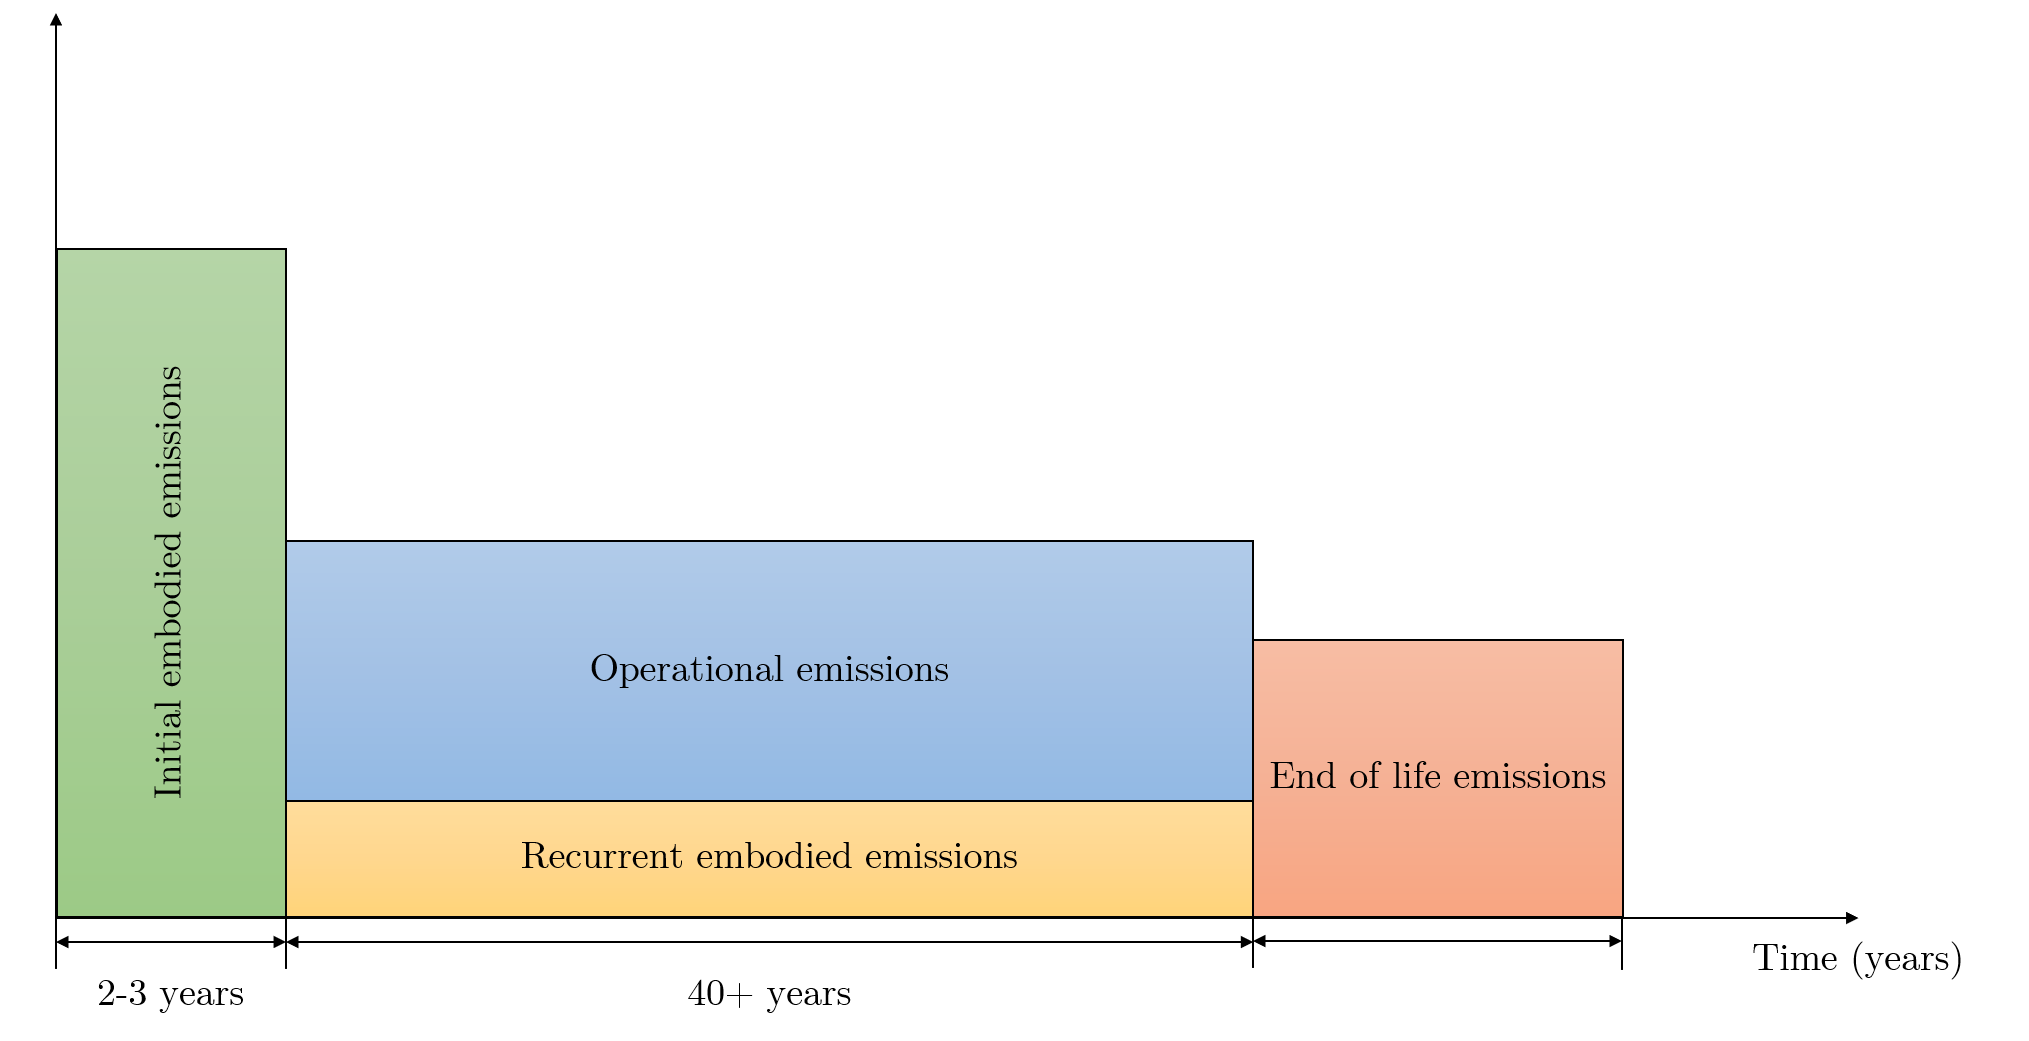
\includegraphics[width=0.85\textwidth]{Figures/LifecycleEmissions.png}
    \caption{Life cycle emissions of a building. Reproduced here from a similar figure originally produced by \citet{Ibn-Mohammed2013-wu}}
    \label{fig:lifecycleemissions}
\end{figure}

\paragraph{} \citet{Hamilton-MacLaren2009-pt} and \citet{Moncaster2012-xm} both conclude that current estimates of embodied energy vary significantly due to large variations in methodology and quality of data. \citet{Koezjakov2018-qw} reported that embodied emissions accounted for 10-12\% of total life cycle emissions for a standard house, rising to 36-46\% for an energy efficient home, due to a decrease in operational emissions. \citet{Chastas2018-zl} analysed 95 individual cases to identify how embodied carbon emissions compared. Values ranged from 9-80\% of the total emissions, with such a wide range still existing even after normalisation to increase the homogeneity and comparability of the sample. The reasons for the deviation were cited as differences in electricity mix and overall building design, amongst others. In a similar study, \citet{Ramesh2010-wc} found that embodied emissions accounted for 10-20\% of total emissions when considering 46 different case studies and noted a positive linear relationship between operational and embodied emissions over a building's lifetime. By focusing on the construction, operation and demolition of two residential buildings in Turkey, \citet{Atmaca2015-dq} found that embodied energy accounted for 24-27\% of overall life cycle consumption. The variation in results here is clear to see, despite many studies considering similar cases. A major factor contributing to the variation is the reliance of operational emissions on the conditions in which the building exists. Even when accounting for this, \citet{Karimpour2014-oj} reported values of embodied energy between 7\% and 42\% of total life cycle energy. \citet{Dixit2019-bj} noted that the ``biggest impact of accuracy and specificity of embodied energy calculations comes from data quality". Hence this is perhaps the most significant factor behind the variation in results. 

\paragraph{} \citet{Hamilton-MacLaren2009-pt} suggest that comparing percentage values can be misleading and hence it is often more relevant to compare absolute values or per-unit values. \citet{Suzuki1995-ve} found the energy due to housing construction in Japan to be between 3-10 GJ/m\textsuperscript{2} depending on the materials used and the size of the dwelling. The same paper reported related CO\textsubscript{2} emissions resulting from initial construction to be between 250 and 850 kg/m\textsuperscript{2}. \citet{Asif2007-sx} performed a life cycle assessment of a 3-bedroom semi-detached house in Scotland and estimated the total embodied energy to be 227.4 GJ. This is equivalent to roughly 1.6 GJ/m\textsuperscript{2}, much lower than the range predicted by \citet{Suzuki1995-ve}. In life cycle analysis of a US residential home \citet{Keoleian2000-de} found the total greenhouse gas emissions to be 1,010 tCO\textsubscript{2}e and the use phase to account for 91\% of total energy consumption. This would suggest embodied CO\textsubscript{2} emissions to be 400 kg/m\textsuperscript{2}, agreeing well with results above despite significant differences in method and studied dwellings. \citet{The_Committee_on_Climate_Change2008-xn} estimated a typical 2-bedroom home in the UK built with new materials to embody around 80 tCO\textsubscript{2}, hence predicting an intensity of roughly 800 kgCO\textsubscript{2}/m\textsuperscript{2} when combined with data on the average floor space of English homes published by the \citet{Department_for_Communities_and_Local_Government2015-rv}. Again, this value is roughly consistent with others, although the bounds suggested by \citet{Suzuki1995-ve} are widely spaced. Whilst absolute values may convey a truer story about the embodied emissions of any single case, they still lack any significant context within the sector as a whole. 

\paragraph{}
The issue of units must also be raised, with some reports detailing embodied energy calculations and others embodied emissions. Embodied energy is an estimation of the energy spent from the time of extraction until the time it reaches its end-use site which, in the case of housing, would be the site of the actual dwelling. Due to the number of variables involved, values of embodied energy vary from study to study. The US Department of Energy’s Buildings Energy Data Book, prepared by \citet{DR_International_Ltd2012-td} is one example of an attempt to aggregate this data, although accuracy is still not guaranteed. \citet{Lushnikova2016-kl} define embodied emissions as the accumulated greenhouse gases caused by a product during its life cycle. Whilst there is an understanding of how the two relate, differences in the methodology used to calculate them do not always allow direct comparisons. Hence, an understanding of the underlying methods behind any quoted values must be considered when comparing the two.

\paragraph{}
Other studies have looked at embodied and operational emissions from a different viewpoint, with \citet{Copiello2017-hm} showing that embodied energy in building products is a positive logarithmic function of product cost. It could be argued that embodied energy should play a more substantial role in wealthier countries, where materials are likely to be of better quality and hence more expensive. On the other hand, wealthier countries are also more able to spend on space-heating and other contributors to operational emissions and hence the relationship is not a simple one. It is also important to note that whilst they are not directly linked, embodied and operational emissions can impact one another. \citet{Filchakova2009-zi} concluded that an increase in renovation rates, and therefore recurrent embodied emissions, does lead to lower in-use energy consumption. Whilst innovation and technological advances have led to reductions in operational emissions in buildings, these measures often lead to an increase in material requirements and hence an increase in embodied energy \citep{Ibn-Mohammed2013-wu}. \citet{Seo2017-uk} found that a 36\% reduction in energy consumption required a 7\% increase in total embodied energy, whilst a 76\% reduction in consumption required a 50.3\% increase in embodied energy. \citet{Ramesh2010-wc} found that too much use of active and passive features often has the opposite effect however, with low energy buildings observed to perform better than self-sufficient (zero operating energy) buildings over the whole life cycle. Since all these conclusions are drawn for specific cases, no wider conclusion can be drawn without comparison with many more results. A more widely applicable method for calculating embodied and operational emissions would facilitate well-informed decision making as to where the optimum lies. 

\subsection{Initial vs. recurrent embodied emissions}
\label{InitialVsEmbodied}

\paragraph{}
Having identified embodied emissions as an area of interest, it is important to understand its component parts. \citet{Dixit2019-bj} states that, broadly speaking, embodied emissions can be split into initial embodied emissions, due to the materials involved in the original construction of the dwelling, and recurrent embodied emissions in the processes of maintenance, repair and replacement. Comparisons between the two sources of emissions in the past have again resulted in some ambiguous results. \citet{Wiedenhofer2015-wn} found that when looking at material flows in the EU, expansion of the housing stock required almost three times the material that maintenance of residential buildings did. More narrow-scoped case studies, such as that by \citet{Barnes1975-jh}, assumed annual recurrent embodied energy to be 0.9\% of initial embodied energy, whilst \citet{Stephan2011-sd} assumed an even lower contribution at just 0.5\%. Significant discrepancies again prevent true comparison between results. 

\paragraph{}
\citet{Dixit2019-bj} performed a systematic survey of literature to identify parameters used in recurrent embodied energy calculations and concluded that, whilst some parameters can be controlled through careful selection of which materials and products to consider, others are uncontrollable and hence will lead to differing results. Due to this inevitable variability, it is hard to justify the scalability of individual cases and hence, when studying the housing stock as a whole, determining the initial and recurrent energy through narrow case studies is likely to be unreliable. It is therefore of interest to consider the stock more generally if wider conclusions are to be drawn.

\subsection{Calculating embodied emissions}
\label{CalculatingEmissions}

\paragraph{}
In calculating embodied emissions, past studies have separated initial and recurrent emissions. Initial embodied emissions are generally calculated using the material requirements of the original build phase whereas attempts to calculate recurrent embodied emissions tend to be more varied. \citet{Dixit2019-bj} found the most commonly used parameter in calculating recurrent embodied emissions to be the service life of relevant components. Determining service life data is hard due to the number of factors affecting it, with \citet{Grant2013-oq} noting that the majority of sources are incomparable due to geographical and temporal differences. As part of a wider study on recurrent embodied energy, \citet{Dixit2019-bj} collated data from 31 different studies to determine the service life of commonly used building materials. The data presented in that study agrees well with that given by \citet{Beobachter_undated-vh}, the \citet{Carbon_Leadership_Forum2018-iq}, the \citet{Royal_Institution_of_Chartered_Surveyors2017-si}, \citet{InterNACHI2019-ae} and \citet{Fannie_Mae2014-ne}, none of which were included in the original study.

\paragraph{}
Once material requirements have been identified, they can be converted to embodied carbon or embodied energy using an appropriate database, such as the one described by \citet{Hammond2008-np}. The values in the database are given as representative of UK construction materials and hence are relevant to this study. According to \citet{Christoforou2016-ye}, cradle to-site embodied energy is defined as the energy used for raw material extraction, production and transportation of the end-product to site. \citet{Hallquist1978-kf} provides an example of how values for the energy use in manufacture of certain materials may be calculated in practice, although it is noted that available data are scarce and uncertain. Data is also published by some manufacturers in the form of an Environmental Product Declaration (EPD). \citet{Moncaster2012-xm} highlight the importance of selecting an appropriate data source for this step since there are inherent inaccuracies in the methodologies used to calculate embodied energy and carbon and hence each data set is limited in its scope and relevance.

\subsection{Analysis of material flows}
\label{materialflows}

\paragraph{}
Whilst much of the work done in this area in the past has been on generating bottom-up estimates of embodied emissions, it should also be possible to arrive at the same number using a top-down approach. By examining material flows within the UK, such as that proposed for the flow of cement by \citet{Shanks2019-nu}, a value for total material usage in the residential sector can be reached. A wider reaching study by \citet{Sheerin2002-aj} accounts for multiple material flows, including imports and exports. That the analysis is possible does not guarantee accuracy, however. Assumptions must be made to separate aggregated data into residential and commercial sectors, as well as complexities involved with estimating proportions of initial and recurrent embodied energy.

\subsection{Identifying a gap in previous literature}

\paragraph{}
As highlighted in the above sections, there are many one-off studies on operational, initial embodied, and recurrent embodied emissions however many of them lack context. Whilst individual studies can be compared to each other, it is hard to provide wider context without an understanding of the scale of emissions for the stock as a whole. If this were to exist, it would provide an easy way to benchmark specific projects against a relevant 'average' case. This would also allow the identification of specific areas of interest when focusing on future policy and targets for the sector. This paper will therefore look to draw on the methods highlighted from previous literature to calculate the initial and recurrent embodied emissions of the English housing stock as a whole. It is hoped that its conclusions may be more relevant to future policy decisions and more representative of the stock as a whole than any previous individual case study.

%---------------------------------------
% Methods
%---------------------------------------

\section{Methods}
\label{methods}

\paragraph{}
This section details the methods used to calculate the annual embodied emissions of the material inputs to the English housing stock. As noted in Section \ref{PreviousLiterature}, it is possible to approach this problem using either a top-down approach, making use of aggregated data and broad assumptions about how the material requirements of different sectors compare, or a bottom-up approach, detailing specific changes to the stock, their frequency, and their material requirements. A wider availability of granular data and its prevalence in previous studies informed the decision to approach this problem using a bottom up approach. In addition to this, the difficulties involved with segmenting aggregated data would potentially introduce unjustifiable uncertainty in results through a top-down approach. In designing the methodology for this study, a key priority was to track uncertainties and errors throughout the analysis. In this regard, it was thought that a top-down approach would have involved assumptions involving errors harder to quantify, hence reducing confidence in the results. 

\paragraph{}
In order to quantify the embodied emissions associated with material inputs to the English housing stock, the frequency of material intensive changes to the stock were explored, along with related material requirements. Planning application data was chosen as a reliable source to help estimate the rate at which different construction works occur. In the year ending December 2016, planning authorities granted 382,600 decisions \citep{Department_for_Communities_and_Local_Government2017-tj}. It was deemed unnecessary to attempt to analyse the whole data set and hence an initial analysis was performed on the housing stock of Cambridgeshire for the year of 2016, due to the availability of comprehensive data for that period. The results drawn from the Cambridgeshire area were then extrapolated to derive results for the English housing stock as a whole. This can be summarised by Equation 1 below.

\begin{equation}
    \text{Total embodied carbon emissions, } C=\sum_{i=1}^{a} \sum_{j=1}^{b} N_i M_{ij} E_j
\end{equation}

\noindent
Where $N_i$ is the number of times a certain material intensive change to the stock $i$ takes place in a given year, $M_{ij}$ is the material $j$ required for change $i$ and $E_j$ is the embodied carbon of material $j$. 

\paragraph{}
In defining each of these variables, therefore, it was possible to quantify the total embodied emissions in the English housing stock. A summary of the method used in this report is given in Figure \ref{fig:flowchart}.

\begin{figure}[!htp]
    \centering
    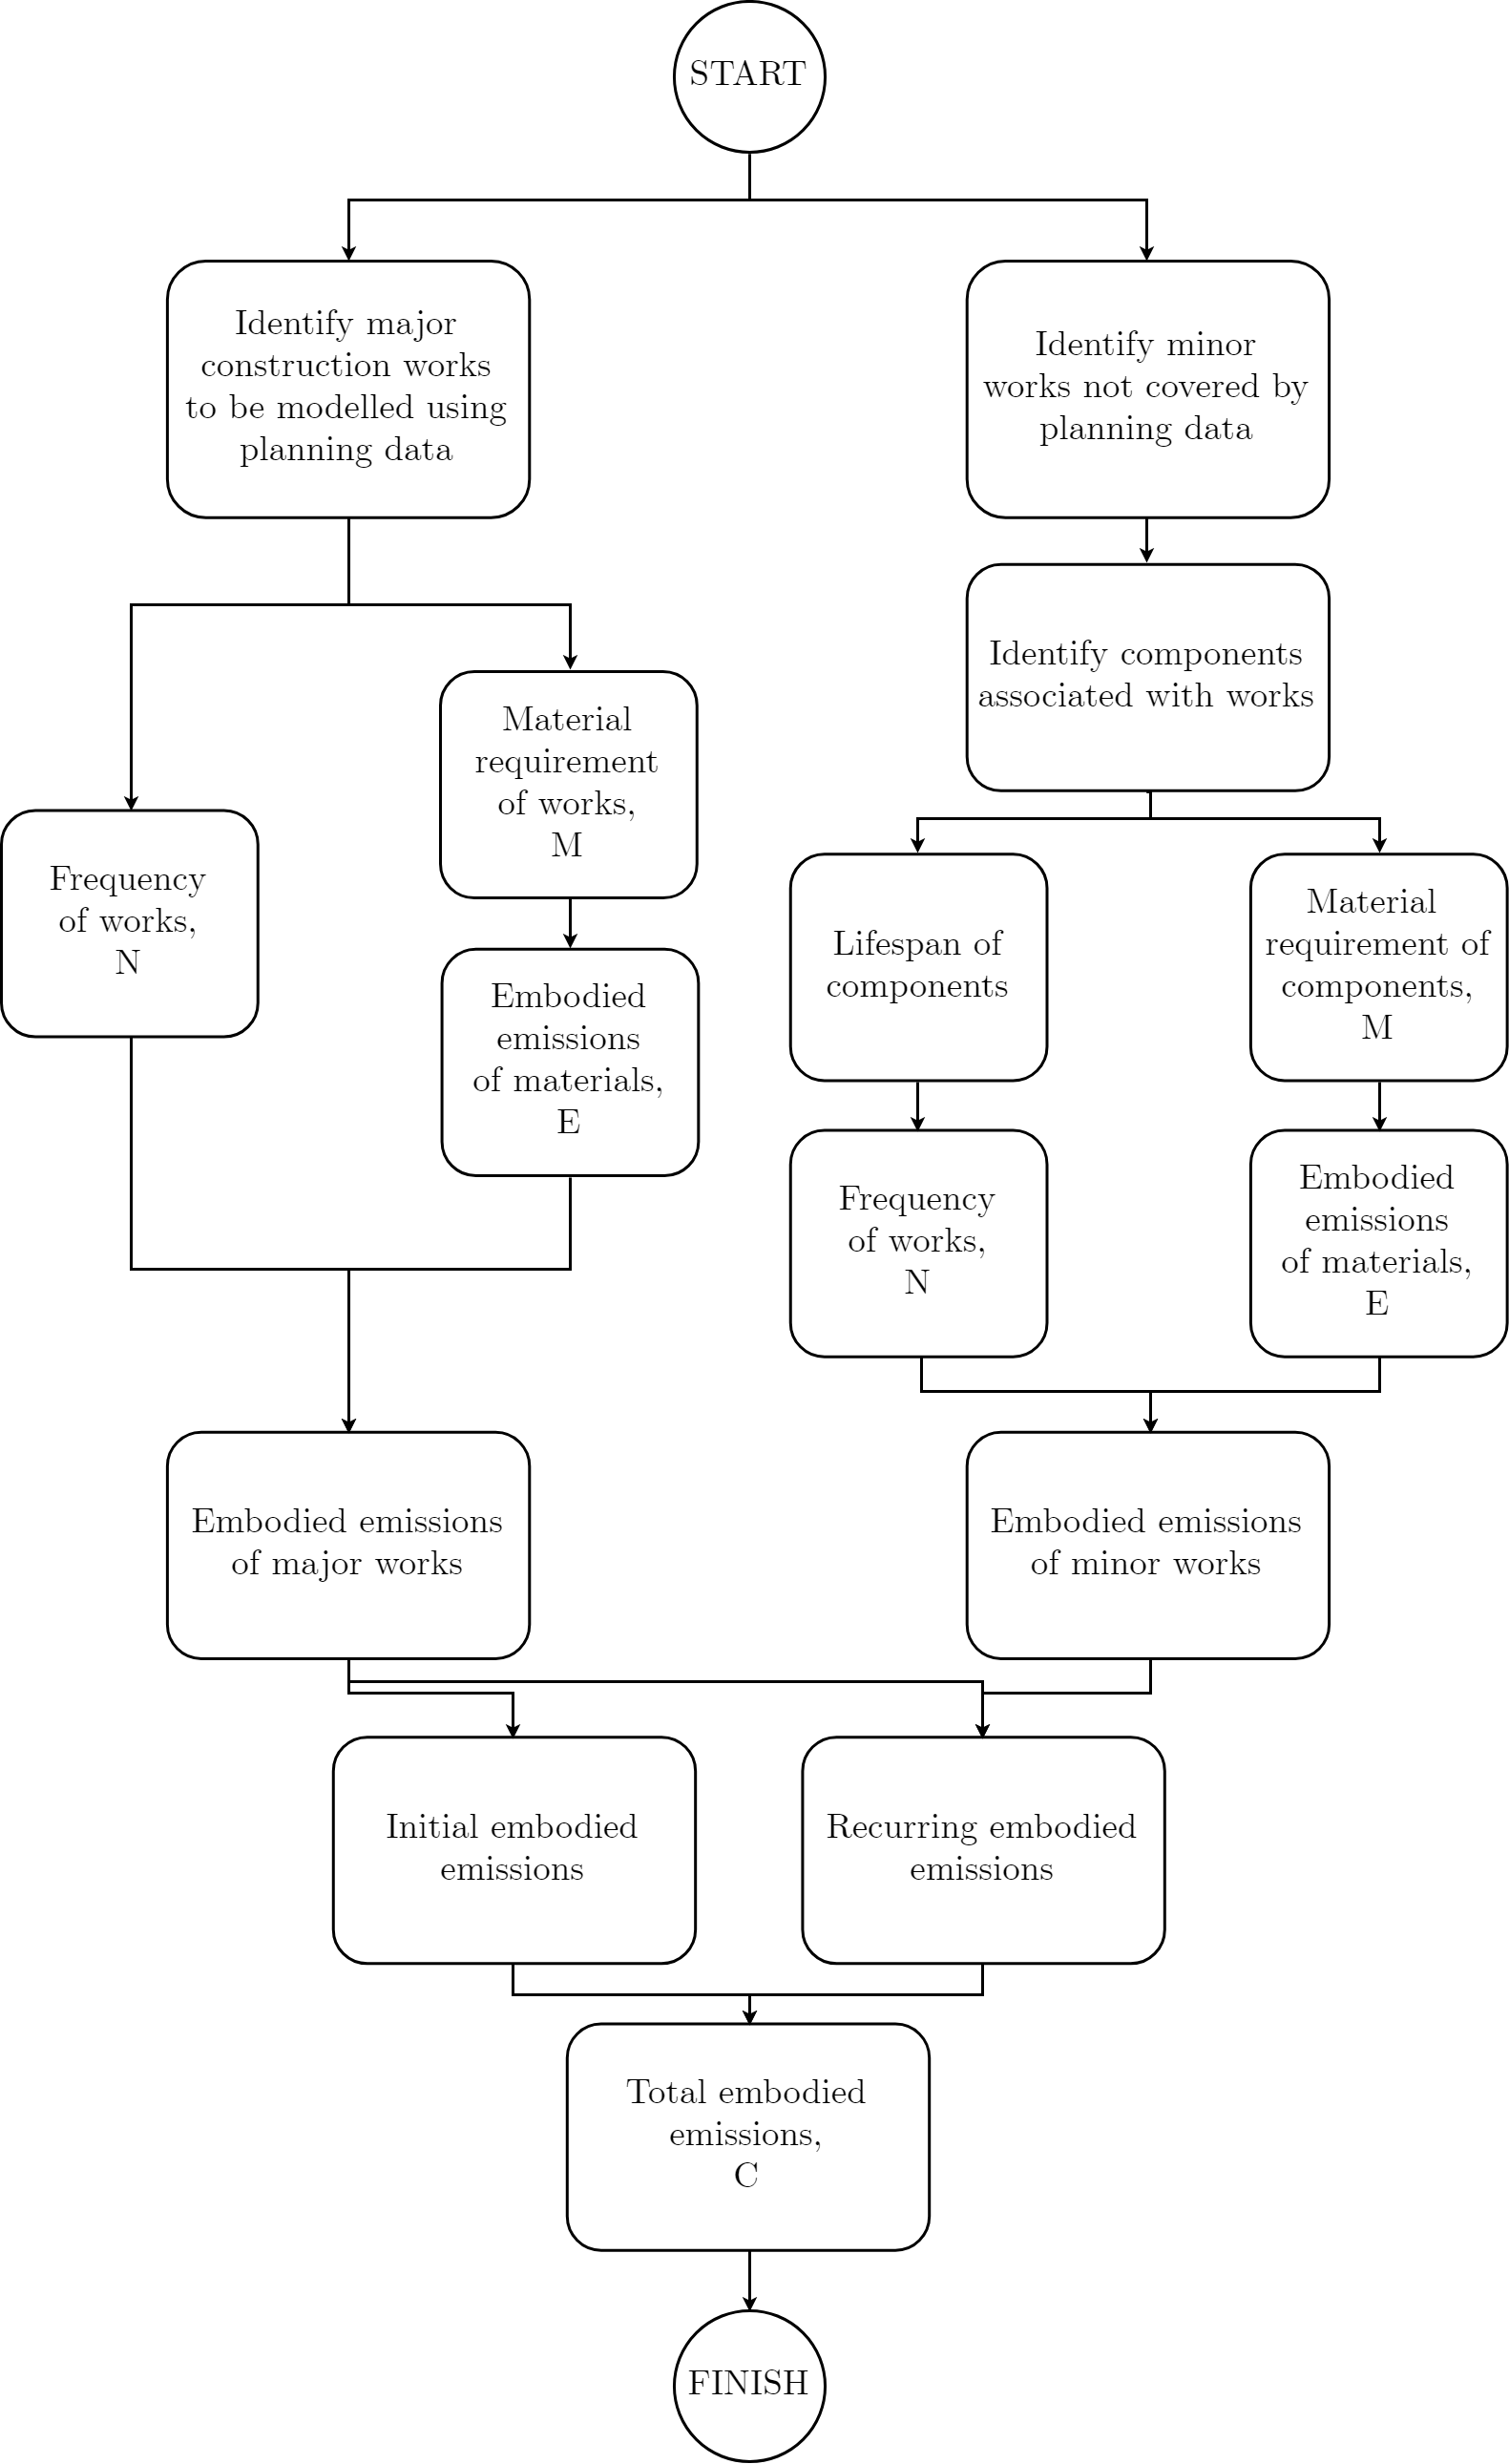
\includegraphics[width=0.78\textwidth]{Figures/Flowchart3.png}
    \caption{A flowchart summarising the methods used in this report to estimate the embodied emissions associated with the annual material input to the English housing stock}
    \label{fig:flowchart}
\end{figure}


\subsection{Estimating the frequency of construction works}
\label{FreqOfWorks}

\paragraph{}
The frequency with which the housing stock is subject to different types of construction work was the first variable to be considered, since it indirectly informed the derivation of the other two. Two separate methods were used to predict the frequency of construction works, largely due to differing availability of relevant data. Planning application data was used in order to assess the frequency of large construction works, such as newly built dwellings, other additions to the stock such as extensions and conservatories, and larger refurbishment works. For smaller refurbishment works not seen in planning application data, or for those for which the planning application data was considered to be insufficient, service life data for relevant components of housing was used to predict a frequency of regeneration.

\subsubsection{Frequency of major works}
\label{FreqMajor}

\paragraph{}
In order to assess the frequency with which different construction works were performed in Cambridgeshire, data was obtained from the website UK PlanIt \citep{Speakman_undated-sd}. UK PlanIt is a national aggregator for current and historical planning information, with data from 98\% of planning authorities in the UK. The Cambridgeshire area includes five independent planning authorities (Cambridge, East Cambridgeshire, Fenland, Huntingdonshire and South Cambridgeshire) and data was collected from all of these.

\paragraph{}
The data obtained was very wide ranging and included more than was for required for this investigation. To that end, all data relating to commercial construction as well as any relating to works of negligible material input were disregarded. Each application has an associated description, which details the purpose of the application and the proposed work. After discarding non-useful entries, each remaining entry was manually tagged by reading the related description. The results of this step were as shown in Table \ref{tab:RelevantCases}, with the frequency recorded as the number of times that particular type of work was successfully applied for in Cambridgeshire in 2016.

\begingroup
\linespread{1}
% Table generated by Excel2LaTeX from sheet '1'
\begin{sidewaystable}[htbp]
  \centering
  \caption{A summary of the successful planning applications in Cambridgeshire in 2016}
    \begin{tabular}{l c C{0.12\textwidth} C{0.13\textwidth} L{0.35\textwidth} c}
    \toprule
    \textbf{Application type} & \textbf{Count} & \textbf{Proportion of total cases} & \textbf{Material requirements} & \textbf{Qualitative material requirements} & \textbf{Include?} \\
    \midrule
    Extensions & \multicolumn{1}{r}{1,477}  & \multicolumn{1}{r}{56.4\%} & High  & Full construction work (walls, floors, roof, foundations etc.) & Y \\
    New houses & \multicolumn{1}{r}{926}   & \multicolumn{1}{r}{35.4\%} & High  & Full construction work & Y \\
    New flats & \multicolumn{1}{r}{751}   & \multicolumn{1}{r}{28.7\%} & High  & Full construction work & Y \\
    New garages & \multicolumn{1}{r}{335}   & \multicolumn{1}{r}{12.8\%} & High  & Full construction work & Y \\
    Change of use & \multicolumn{1}{r}{234}   & \multicolumn{1}{r}{8.9\%} & Low   & Fixtures \& fittings, minimal structural work & N \\
    Small outbuildings &\multicolumn{1}{r}{134}   & \multicolumn{1}{r}{5.1\%} & Mid   & Wooden/other standalone structure & Y \\
    Conversion & \multicolumn{1}{r}{106}   & \multicolumn{1}{r}{4.0\%} & Low   & Fixtures \& fittings, minimal structural work & N \\
    Roofs & \multicolumn{1}{r}{93}    & \multicolumn{1}{r}{3.6\%} & Low   & Tiles and or supporting structure & N \\
    Porches & \multicolumn{1}{r}{91}    & \multicolumn{1}{r}{3.5\%} & Low   & Small extension to front of house & N \\
    Windows & \multicolumn{1}{r}{76}    & \multicolumn{1}{r}{2.9\%} & Low   & Glazing & N \\
    Garage conversions & \multicolumn{1}{r}{75}    & \multicolumn{1}{r}{2.9\%} & Low   & Fixtures \& fittings, minimal structural work & N \\
    Conservatories & \multicolumn{1}{r}{72}    & \multicolumn{1}{r}{2.8\%} & Mid   & Glazed structures requiring foundations & Y \\
    Fencing & \multicolumn{1}{r}{71}    & \multicolumn{1}{r}{2.7\%} & Low   & Low complexity masonry or wooden structure & N \\
    Loft conversions & \multicolumn{1}{r}{70}    & \multicolumn{1}{r}{2.7\%} & Low   & Fixtures \& fittings, minimal structural work & N \\
    Insulation/Rendering & \multicolumn{1}{r}{44}    & \multicolumn{1}{r}{1.7\%} & Low   & Plaster or pre-manufactured boards/roll & N \\
    Car ports & \multicolumn{1}{r}{38}    & \multicolumn{1}{r}{1.5\%} & Mid   & Non-enclosed wooden/metal shelter & N \\
    Balconies & \multicolumn{1}{r}{30}    & \multicolumn{1}{r}{1.1\%} & Low   & Brickwork and metal fixtures & N \\
    Doors & \multicolumn{1}{r}{22}    & \multicolumn{1}{r}{0.8\%} & Low   & Small amounts of wood and glazing & N \\
    Chimneys & \multicolumn{1}{r}{4}     & \multicolumn{1}{r}{0.2\%} & Low   & Brickwork & N \\
    \midrule
    Total relevant cases & \multicolumn{1}{r}{2618}  &       &       &       &  \\
    \bottomrule
    \end{tabular}%
  \label{tab:RelevantCases}%
\end{sidewaystable}%
\endgroup

\paragraph{}
By considering the relative frequency together with a qualitative estimate of material requirements, it was possible to narrow down which application types should be taken forward for further analysis. The applications that were not analysed further were rejected either on the basis that they did not occur with enough frequency, or that their associated material requirements were small when compared with other works. The majority of application types rejected in this step however, were accounted for in the analysis of refurbishment as detailed in Section \ref{refurb}. Due to the large number of related applications, it was decided to segment certain application types as follows:

\begin{itemize}
\itemsep0em
    \item New houses into two and three storey
    \item New flats into studio, one-bed, two-bed, three-bed, and four-bed
    \item Garages into single, double, and triple
    \item Extensions into one-storey, two-storey, and three-storey 
\end{itemize}

\paragraph{}
Segmentation of conservatories and small outbuildings was not required due to the variation in proposed works being relatively small. In analysing the data this way, some uncertainty was introduced in cases where data was incomplete (e.g. a new build house with an unspecified number of storeys). To account for this, when aggregating data, three different estimates were produced that corresponded to low, mid, and high material input for each construction work.

\subsubsection{Frequency of minor works}
\label{FreqMinor}

\paragraph{}
Since many minor refurbishment works are not included in planning application data, they needed to be modelled using a different method to that described above. Minor refurbishments were assumed to be the replacement of components which have come to the end of their useful life, rather than the addition of any new material, which is almost impossible to model (apart from that seen in planning data). Service life data such as that proposed by \citet{Dixit2019-bj} was used to estimate the rate of regeneration of certain components of housing.

\paragraph{}
The decreasing rate of demolition of English housing, along with the relatively low absolute values of losses compared with stock additions, led to the assumption that the effects of demolition or finite life can be ignored. If it is assumed that houses are constructed at a constant rate, then it should follow that the age distribution of the housing stock is approximately even. \citet{Adams2008-ae} point out that fluctuations are seen due to Government policy, supply of land and many other variables, however these tend to by cyclical and so can be assumed to not affect the distribution when averaged over a longer period. With a flat age distribution within the English housing stock, it was then estimated that the rate of refurbishment within the stock is constant and hence the replacement of components can be summarised as in Equation 2.

\begin{equation}
    N_i = \frac{1}{L_i}
\end{equation}

\noindent
Where $N_i$  is the proportion of all components $i$ replaced each year and $L_i$ is estimated lifespan of component $i$.

\paragraph{}
The relevant components to be considered in this way were identified as:

\begin{multicols}{2}
\begin{itemize}
\itemsep0em
	\item Interior and exterior doors
	\item Roofing
	\item Brickwork
	\item Concrete blocks
	\item Glass
	\item Timber
\end{itemize}
\end{multicols}

\paragraph{}
Other components were excluded on the basis that the relative amount of material in the stock to be replaced is negligible, or that the life span of the component is assumed so large that its effect in any one year is small compared to those considered. Just as for the major construction works, the service life data employed here has its limitations, and hence minimum, maximum and mean values of service life reported in data were used, as shown below in Table \ref{tab:Lifespans}.

\begingroup
\linespread{1}
% Table generated by Excel2LaTeX from sheet '2'
\begin{table}[htbp]
  \centering
  \caption{A summary of relevant service life data as quoted by \citet{Dixit2019-bj}}
    \begin{tabular}{lccccc}
    \toprule
    \textbf{Component} & \textbf{Maximum} & \textbf{Minimum} & \textbf{Median} & \textbf{Mean} & \textbf{Std. Dev.} \\
    \midrule
    Indoor doors & 50    & 15    & 30    & 32    & 17 \\
    Exterior doors & 100   & 19    & 40    & 45    & 28 \\
    Roofing/Asphalt Roofing & 60    & 15    & 30    & 33    & 15 \\
    Brick & 120   & 50    & 90    & 84    & 41 \\
    Concrete Blocks & 120   & 50    & 80    & 79    & 40 \\
    Glass/Glass panels & 40    & 25    & 40    & 36    & 12 \\
    Timber & 90    & 37    & 55    & 59    & 21 \\
    \bottomrule
    \end{tabular}%
  \label{tab:Lifespans}%
\end{table}%
\endgroup

\subsection{Material requirements of construction works}
\label{MaterialReqs}

For each of the different types of construction work detailed in Section \ref{FreqOfWorks} a bill of materials (BOM) was estimated. As identified in the \citet{nhbc_2015-cg} report titled ‘Homes through the decades’, the key components of housing are roofing, walls, windows, flooring and foundations. Whilst construction techniques have changed a lot over the past century, the materials used have not progressed in the same way. A large proportion of houses in the English housing stock have been, and continue to be, built with the following characteristics:

\vspace{2mm}
\begingroup
\linespread{1}
% Table generated by Excel2LaTeX from sheet '3'
\begin{table}[htbp]
  \centering
    \begin{tabular}{L{0.19\textwidth} L{0.75\textwidth}}
    \textbf{Roofs:} & Concrete tiles sitting on a wooden truss \\
    \textbf{Exterior walls:} & Cavity walls with inner concrete block layer and outer brick layer \\
    \textbf{Interior walls:} & Solid walls made from concrete blocks \\
    \textbf{Windows:} & Double glazing \\
    \textbf{Floors:} & Concrete ground floor and wooden upper floors \\
    \textbf{Foundations:} & Concrete trench foundation \\
    \end{tabular}%
  \label{tab:Characteristics}%
\end{table}%
\endgroup

\vspace*{-7mm}

\paragraph{}
For this reason, the BOM models were developed considering six specific construction materials and it was assumed that the housing stock is built exclusively using the characteristics detailed above. The materials considered in this report are as follows:

\begin{multicols}{2}
\begin{itemize}
\itemsep0em
    \item Brick
	\item Concrete blocks
	\item Concrete tiles
	\item Poured concrete
	\item Wood
	\item Glass
\end{itemize}
\end{multicols}

\paragraph{}
In order to accurately model the material requirements for each different type of construction work, the size of each different work had to be quantified. For this, average floor space statistics for the English housing stock were used. The \citet{Department_for_Communities_and_Local_Government2015-rv} publishes minimum gross internal floor area requirements for different dwelling types. This data is segmented by number of bedrooms, number of bed spaces, and number of storeys and hence provides more specific data than is required for the models being developed here. The number of bed spaces is indicative of the number of people that can be accommodated within the bedrooms of a dwelling and hence is not a directly useful indicator of dwelling size for this particular study. A similar data set included in the Homes and Communities Agency’s Housing Quality Indicators, part of the \citet{The_National_Affordable_Homes_Survey2008-cv}, reports slight variations in the data proposed by the Department for Communities and Local Government and hence the two data sets could be combined to give Table \ref{tab:Floorspace}.

\begingroup
\linespread{1}
% Table generated by Excel2LaTeX from sheet '4'
\begin{table}[htbp]
  \centering
  \caption{Minimum, average and maximum gross floor area data used for developing BOM models}
    \begin{tabular}{lccc}
    \toprule
    \textbf{Designed Occupancy} & \multicolumn{3}{c}{\textbf{Gross Floor Area (m\textsuperscript{2})}} \\
          & \textit{Minimum} & \textit{Mean} & \textit{Maximum} \\
    \midrule
    \textit{1 storey} &       &       &  \\
    \quad Studio & 30    & 34.5  & 39 \\
   	\quad 1 bedroom & 45    & 47.5  & 50 \\
    \quad 2 bedrooms & 57    & 66    & 75 \\
    \quad 3 bedrooms & 67    & 81    & 95 \\
    \quad 4 bedrooms & 75    & 96    & 117 \\
    \textit{2 storeys} &       &       &  \\
    \quad 2 bedrooms & 67    & 73    & 79 \\
    \quad 3 bedrooms & 67    & 84.5  & 102 \\
    \quad 4 bedrooms & 82    & 103   & 124 \\
    \textit{3 storeys} &       &       &  \\
    \quad 3 bedrooms & 85    & 96.5  & 108 \\
    \quad 4 bedrooms & 85    & 107.5 & 130 \\
    \quad 5+ bedrooms & 115   & 126.5 & 138 \\
    \bottomrule
    \end{tabular}%
  \label{tab:Floorspace}%
\end{table}%
\endgroup

\paragraph{}
These values were used to generate the BOM models for each identified construction work. The low, mid, and high values allowed limits to be placed on the error in each calculation. Each model was generated in a similar way, by using floor space to calculate the volumes of material required as follows:

\begin{itemize}
\itemsep0em
    \item Room dimensions could be calculated by combining floor space data with the number of rooms assumed to be in each type of dwelling
	\item With room dimensions set, interior and exterior wall area could be estimated and used to derive the number of bricks and blocks required for the construction work
	\item Roof area was assumed to be equal to floor area, from which the number of roof tiles required can be estimated
	\item The foundation was assumed to be a trench of constant width and depth, and of a length equal to the perimeter of the construction work
	\item The ground floor was assumed to be concrete, with subsequent floors made of timber
	\item The window area was assumed to be a fixed percentage of the floor space
\end{itemize}
	
\paragraph{}
Such that this standardised model could be used, certain assumptions on dimensions were made, summarised in Table \ref{tab:assumptions} with their respective sources. 

\begingroup
\linespread{1}
% Table generated by Excel2LaTeX from sheet '5'
\begin{table}[htbp]
  \centering
  \caption{Main assumptions used throughout the derivation of BOM models}
    \begin{tabular}{l L{0.27\textwidth} c L{0.4\textwidth}}
    \toprule
    \textbf{Component} & \textbf{Assumption} & \textbf{Value} & \textbf{Source} \\
    \midrule
    Walls & Storey height (m) & 3.2   & \textit{\citet{Opdc2018-mp}} \\
          & Exterior wall bricks (per m\textsuperscript{2}) & 60    & \textit{diydata.com, Jewson, Screwfix} \\
          & Exterior wall blocks (per m\textsuperscript{2})  & 10    & \textit{diydata.com, Ridgeons, Screwfix} \\
          & Internal wall blocks  (per m\textsuperscript{2}) & 10   & \textit{diy-extra.co.uk, Ridgeons, Screwfix} \\
    Floor & Ground floor depth (m) & 0.15  & \textit{concreteconstruction.net, designingbuildings.co.uk} \\
          & Upper floor depth (m) & 0.036 & \textit{B\&Q, woodandbeyond.com} \\
    Roof  & Roof tiles (per m\textsuperscript{2}) & 60    & \textit{roofingsuperstore.co.uk, roof-stores.co.uk} \\
    Foundation & Foundation depth (m) & 2     & \textit{designingbuildings.co.uk, self-build.co.uk, homebuilding.co.uk} \\
          & Foundation width (m) & 0.5   & \textit{designingbuildings.co.uk, self-build.co.uk, homebuilding.co.uk} \\
    Windows & Glazing area/floor area & 0.15  & \textit{\citet{US_Environmental_Protection_Agency2012-or}} \\
          & Glazing thickness (m) & 0.008 & \textit{replacedoubleglazing.com \citep{Sanderson_undated-yz}, thermawood.com} \\
    Other & Breakages/defects & 10\%  & \textit{diydata.com, homebuilding.co.uk} \\
    \bottomrule
    \end{tabular}%
  \label{tab:assumptions}%
\end{table}%
\endgroup

\subsubsection{New build flats}
\label{newbuildflats}

\paragraph{}
In order to estimate the material requirements of a newly built flat from floor space statistics, certain assumptions must be made as to the shape of the dwelling. Such that each type of dwelling can be modelled in a similar way, all flats were assumed to be square in shape, with a side length equal to the square root of the gross floor area. The process described in Section \ref{MaterialReqs} was then used to derive the relevant material requirements. Each flat was also assumed to have one external door, as well as one internal door per room.

\paragraph{}
The method described in Section \ref{MaterialReqs} assumes each dwelling to be built as a standalone structure. One difference to that method that must be considered here is that, unlike new-build houses, new-build flats are often built as part of a larger development and hence cannot be simply modelled as a one storey dwelling. To account for this, the average number of storeys in a block of flats in England was calculated using data from the 2008 English Housing Survey \citep{Ministry_of_Housing_Communities_and_Local_Government2017-xx}. The effect of larger developments on material input is to reduce the roof area, foundation volume, and ground floor volume. It was therefore assumed that these can be modelled as in Equations 3, 4, and 5. 

\begin{equation}
    \text{Roof area of a flat, } A_r = \frac{A_f}{N_{avg}}
\end{equation}

\noindent
Where $A_f$ is the floor area of the flat and $N_{avg}$ is the average number of storeys in a block of flats in England. 

\begin{equation}
    \text{Foundation volume of a flat, } V_f = \frac{V_{h,eq}}{N_{avg}}
\end{equation}

\noindent
Where $V_{h,eq}$ is the foundation volume for a house of the same footprint and $N_{avg}$ is the average number of storeys in a block of flats in England. 

\begin{equation}
    \text{Ground floor volume of a flat, } V_g = \frac{V_{g,eq}}{N_{avg}}
\end{equation}

\noindent
Where $V_{g,eq}$ is the ground floor volume for a house of the same footprint and $N_{avg}$ is the average number of storeys in a block of flats in England. 

\paragraph{}
As well as the effects considered above, is it common for the footprint of a block of flats to be larger than any individual flat itself, due to each storey being separated into multiple units. Since no easily accessible data exists on this and variations from development to development would be hard to model, it was assumed that this results only in 50\% of a flat’s external walls being internal with respect to the building. These walls could therefore be assumed to be constructed without the use of bricks and in line with all other internal wall assumptions. The total window area of each flat was also therefore scaled in line with the exterior wall area. Specific assumptions relating to the layout and design of different flats are shown in Figure \ref{fig:flatlayout}, where dashed lines represent the internal walls of each flat type. The actual layout of each type of flat is not critical - these figures are to show assumptions made regarding the internal wall area associated with each.

\begin{figure}[!ht]
     \centering
     \subcaptionbox{Studio flat}{
    	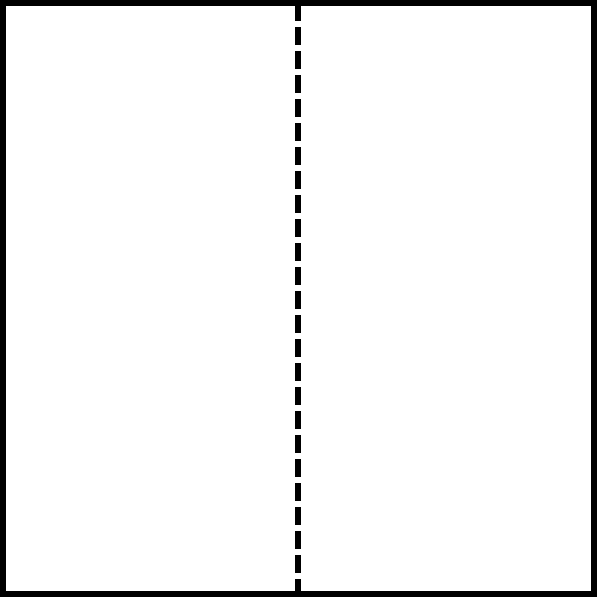
\includegraphics[width=0.3\textwidth]{Figures/Studio_layout.png}
        }
    \subcaptionbox{One-bedroom flat}{
    	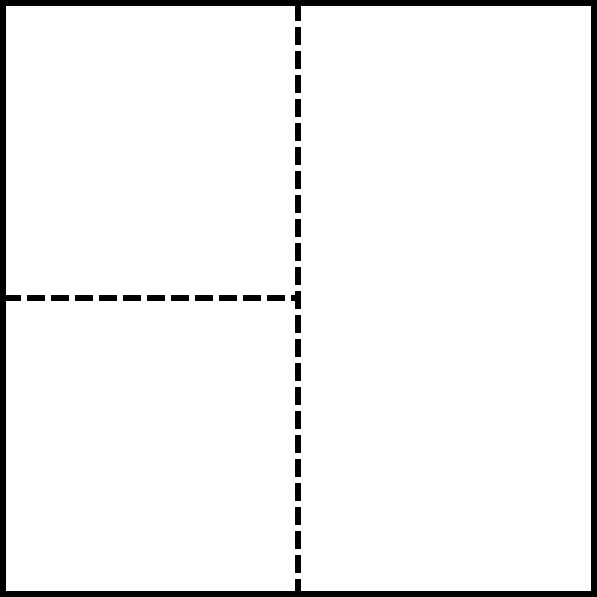
\includegraphics[width=0.3\textwidth]{Figures/1_bed_layout.png}
        }   
    \subcaptionbox{Two-bedroom flat}{
    	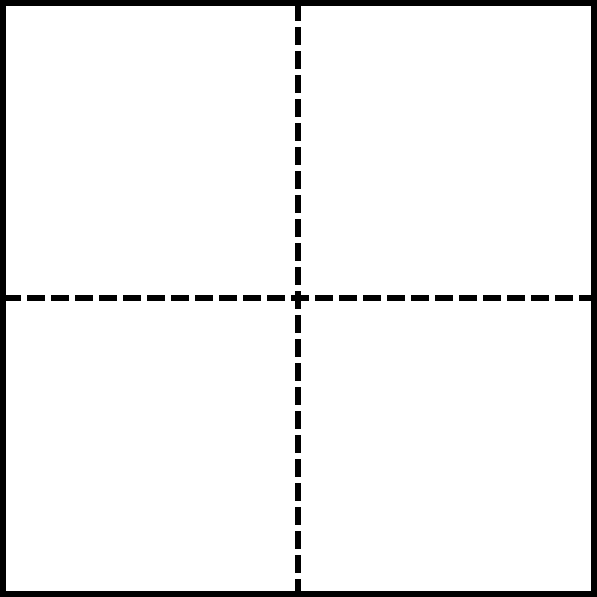
\includegraphics[width=0.3\textwidth]{Figures/2_bed_layout.png}
        }
    \subcaptionbox{Three-bedroom flat}{
    	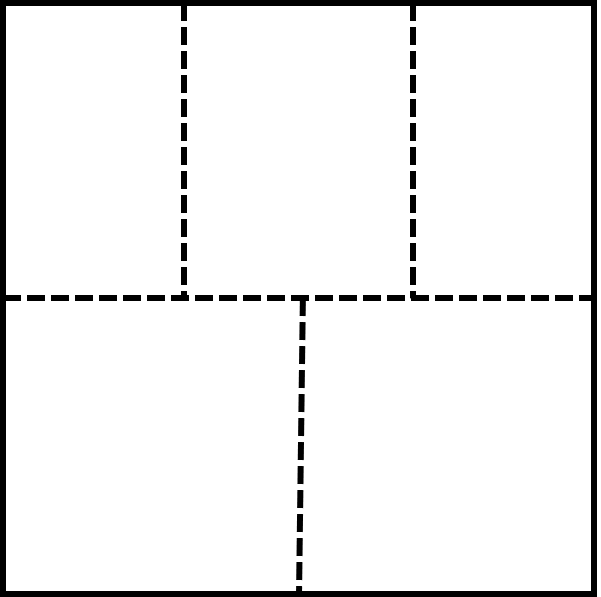
\includegraphics[width=0.3\textwidth]{Figures/3_bed_layout.png}
        }
    \subcaptionbox{Four-bedroom flat}{
    	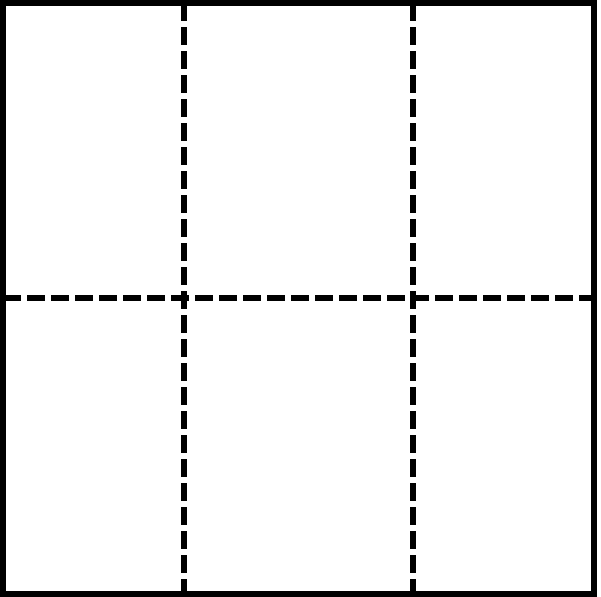
\includegraphics[width=0.3\textwidth]{Figures/4_bed_layout.png}
        }
    \caption{Assumed layout of each flat type for the purpose of developing BOM models}
    \label{fig:flatlayout}
\end{figure}

\subsubsection{New build houses}
\label{newbuildhouse}

\paragraph{}
Just as for new build flats, new build houses were assumed to have a square footprint. They were also assumed to consist of identical storeys. Each storey was assumed to be formed of three rooms, separated by internal walls of length equal to three times the average room side length (similar to the assumption made for a one-bedroom flat). Hence, a two-storey house was assumed to have six rooms and a three-storey house nine. It therefore follows that the perimeter length for two-storey and three-storey houses can be given by Equations 6 and 7, where $A_f$ is the total floor area of the dwelling.

\begin{equation}
    P_{2st} = \sqrt{\frac{A_f}{2}}
\end{equation}

\begin{equation}
    P_{3st} = \sqrt{\frac{A_f}{3}}
\end{equation}

\paragraph{}
The average room side length can also be given by Equations 8 and 9. 

\begin{equation}
    L_{2st} = \sqrt{\frac{A_f}{8}}
\end{equation}

\begin{equation}
    L_{3st} = \sqrt{\frac{A_f}{12}}
\end{equation}

\paragraph{}
Using these values, the material requirements could be calculated as summarised in Section \ref{MaterialReqs}. The number of rooms in each storey is based on 2011 census data \citep{Office_for_National_Statistics2011-wb} which reported the number of rooms in each household. This is shown as a percentage of the whole stock in Table \ref{tab:housecensus}. 

\begingroup
\linespread{1}
% Table generated by Excel2LaTeX from sheet '6'
\begin{table}[htbp]
  \centering
  \caption{Total dwellings in England by number of rooms, as given in 2011 census data \citep{Office_for_National_Statistics2011-wb}}
    \begin{tabular}{lrr}
    \toprule
    \multicolumn{1}{c}{\textbf{Number}} & \multicolumn{1}{c}{\textbf{Dwelling}} & \multicolumn{1}{c}{\textbf{Percentage}} \\
     \multicolumn{1}{c}{\textbf{of rooms}} & \multicolumn{1}{c}{\textbf{count}} & \multicolumn{1}{c}{\textbf{of stock}} \\
    \midrule
    2 or fewer & 813,315 & 4\% \\
    3 & 2,264,602 & 10\% \\
    4 & 4,227,236 & 19\% \\
    5 & 5,446,830 & 25\% \\
    6 & 4,275,834 & 19\% \\
    7 & 2,223,733 & 10\% \\
    8 or more & 2,811,818 & 13\% \\
    \bottomrule
    \end{tabular}%
  \label{tab:housecensus}%
\end{table}%
\endgroup

\paragraph{}
Whilst the most common number of rooms in a household is five, 42\% of households in 2011 had six or more rooms. Taking into account the assumptions made when modelling new build flats as well as new build houses, these produce a similar profile to the one seen in Table \ref{tab:housecensus}, hence providing validation for the assumptions. The comparison of the profiles is presented in Table \ref{tab:profilecomparison}.

\begingroup
\linespread{1}
% Table generated by Excel2LaTeX from sheet '7'
\begin{table}[htbp]
  \centering
  \caption{Comparison of the English housing stock in terms of rooms per dwelling and the modelled stock}
    \begin{tabular}{lrr}
    \toprule
    \multicolumn{1}{c}{\textbf{Number}} & \multicolumn{1}{c}{\textbf{Actual}} & \multicolumn{1}{c}{\textbf{Modelled}} \\
     \multicolumn{1}{c}{\textbf{of rooms}} & \multicolumn{1}{c}{\textbf{profile}} & \multicolumn{1}{c}{\textbf{profile}} \\
    \midrule
    2 or less & 4\%   & 7\% \\
    3 or 4 & 29\%  & 25\% \\
    5 or 6 & 44\%  & 62\% \\
    7 or above & 23\%  & 7\% \\
    \bottomrule
    \end{tabular}%
  \label{tab:profilecomparison}%
\end{table}%
\endgroup

\subsubsection{Extensions}
\label{extensions}

\paragraph{}
Extensions were assumed to extend the house in a single direction by half the footprint side length, based on the average size of extensions seen in practice. Planning permission in England limits the distance by which a single-storey rear extension can extend beyond the original wall of the house to 4 meters if detached and 3 meters for any other house \citep{Garrett2015-bb}. This also agrees with ‘typical’ extension sizes, quoted in a number of articles on the topic, of between 15m\textsuperscript{2} and 35m\textsuperscript{2} \citep{Warwick2019-wt,velux_undated-ea,Searle2018-qb,sterlingbuild_undated-kj,Madsen2012-jm}. The footprint side length was taken as an average of the lengths used in modelling new build houses, resulting in predicted extensions of between 16m\textsuperscript{2} and 31m\textsuperscript{2}. 

\paragraph{}
In line with assumptions from other sections, each extension was considered to have one interior door per room and one exterior door per extension. Two and three storey extensions were assumed to have identical storeys stacked on top of one another. Each storey was assumed to contain two rooms, separated by an interior wall of length equal to half the footprint side length of the original house.

\subsubsection{Garages}
\label{garages}

\paragraph{}
Garages were modelled much like single-storey houses, although the walls were not assumed to use concrete blocks walls since insulation standards are not as high as for housing. Walls were assumed to be formed using two leaves of masonry however, since a single leaf would not provide adequate resistance to rain and could consequently become damp \citep{National_House-Building_Council2011-qi}. 

\paragraph{}
The average size of a garage in the UK, as quoted by multiple sources, is given in Table \ref{tab:garagesize} and these were the dimensions used to calculate the material requirements of each type \citep{buildsearch_2018-gp,eastern_garage_2018-oj,garage_plans_undated-ub,Wikipedia_contributors2019-ik}. Double garages were assumed to have a gross area twice as big as single garages, and triple three times as big.

\begingroup
\linespread{1}
% Table generated by Excel2LaTeX from sheet '8'
\begin{table}[htbp]
  \centering
  \caption{Estimates of garage floor area to be used in BOM models}
    \begin{tabular}{lccc}
    \toprule
          &       & \textbf{Gross floor area (m\textsuperscript{2})} &  \\
    \textbf{Garage type} & \textit{Low estimate} & \textit{Mid estimate} & \textit{High estimate}\\
    \midrule
    Single   & 11.76 & 14.85 & 18.30 \\
    Double & 23.52 & 29.70 & 36.60 \\
    Triple   & 35.28 & 44.55 & 54.90 \\
    \bottomrule
    \end{tabular}%
  \label{tab:garagesize}%
\end{table}%
\endgroup

\paragraph{}
In contrast to the height of dwelling storeys, for a garage to be built under permitted development, it must have a maximum eaves height of 2.5 meters \citep{planning_portal_2015-kr}. Typical garage ceilings are lower than for an interior room, with the minimum recommended garage height 2.1 meters \citep{house_plans_undated-if}. Low, mid, and high estimates of heights were therefore taken as 2.1 meters, 2.3 meters, and 2.5 meters respectively.

\subsubsection{Conservatories}
\label{conservatories}

\paragraph{}
Conservatories were assumed to be similar to single-storey extensions, although they differ in terms of dimensions and materials used. Conservatories tend to have a smaller gross floor area than extensions, with typical sizes ranging from 9m\textsuperscript{2} to 16m\textsuperscript{2} \citep{homeadvice_2019-gc,householdquotes_undated-es,Reed2018-sz}. It was therefore assumed in this study that a conservatory adds an area equal to a quarter of the original house footprint, hence an area of between 8.3m\textsuperscript{2} and 15.3m\textsuperscript{2}.

\paragraph{}
In order to be classified as a conservatory, at least half of the wall area and at least 75\% of the roof area must be glazed or made of a translucent material \citep{ashford_undated-xr}. Other estimates note that conservatories can have up to 80\% glazed surfaces and a fully glazed roof \citep{MyGlazing_undated-ah}. In this case, low, mid, and high estimates of wall glazing were taken as 50\%, 65\% and 80\% respectively, with a fully glazed roof. It was assumed that the remaining wall area is formed in the same way as other external walls.

\subsubsection{Garden rooms}
\label{gardenroom}

\paragraph{}
Garden rooms and other outbuildings, since they are detached from the building to which they belong, are modelled with a method slightly further removed from other construction works. Garden rooms come in a wide variety of sizes, from around 7m\textsuperscript{2} to more than 30m\textsuperscript{2} \citep{apodo_undated-hl}. It was assumed here that the average garden room is sized the same as an average conservatory, at 11m\textsuperscript{2}, although the low and high estimates were adjusted to account for the wide range in available sizes. Just as with garages, permitted development limits garden room height to 2.5m and hence the most popular style in the UK is a 2.5m high flat-roofed garden room \citep{Garden_Room_Guide_2015-is}.

\paragraph{}
Just as with a conservatory, the materials used for garden rooms are not the same as for a usual dwelling. Garden rooms are typically built using wood \citep{Lazy_Susan_2012-ke} and tend to have a higher level of glazing than a usual extension \citep{lomax_undated-od}. As a consequence, this study modelled garden rooms as wooden structures with glazed wall area equal to 30\% of the floor area (double that seen in the average dwelling). 

\paragraph{}
Since garden rooms are not as substantial as regular extensions, they do not require the same foundations. The most common type of garden room foundation is a concrete slab foundation \citep{Garden_room_guide_2009-hx}, with the average thickness of paving slabs taken to be 38mm \citep{Wickes_undated-br}. This value was assumed for the analysis here, and the slabs were assumed to be concrete.

\subsubsection{Refurbishment of dwellings}
\label{refurb}

\paragraph{}
As well as the additions to the housing stock presented above, there is a material requirement associated with refurbishing the existing stock and ensuring it remains fit for purpose. In order to model this, in a similar way to that presented above, BOM models were developed for the annual refurbishment of one, two, and three storey dwellings. For each dwelling type, the quantity of materials required for the initial build phase was derived. From this, as noted in Section \ref{FreqMinor}, a fixed proportion of each relevant material was assumed to be replaced each year, according to its service life. As with each other type of construction work, low, mid, and high estimates were made to provide bounds on the error introduced by assumption. These were calculated using quoted bounds on floor space and service life data.

\subsection{Converting material requirements into embodied emissions}
\label{materialtoemissions}

\paragraph{}
Once the material requirements of each construction work had been derived, the open-access database described by \citet{Hammond2008-np} was used to convert to embodied emissions. In the case where multiple values are given for a material (e.g. timber), the most appropriate value for the application being modelled was selected. In the case of concrete, it is recommended to avoid selecting a `general’ value, since a wide range of values exist with each dependent on the specific make up. In this case, a 12\% cement content by mass was assumed and a concrete type suitable for foundations and ground floors chosen. The resulting conversions factors used are given in Table \ref{tab:emissionsfactors}.

\begingroup
\linespread{1}
% Table generated by Excel2LaTeX from sheet '9'
\begin{table}[htbp]
  \centering
  \caption{Conversion factors used to estimate the emissions associated with each material used in BOM models}
    \begin{tabular}{lc}
    \toprule
    \textbf{Material} & \textbf{kgCO\textsubscript{2}e/kg} \\
    \midrule
    Bricks & 0.24 \\
    Blocks & 0.10 \\
    Tiles & 0.10 \\
    Concrete & 0.15 \\
    Wood  & 0.61 \\
    Glass & 0.91 \\
    \bottomrule
    \end{tabular}%
  \label{tab:emissionsfactors}%
\end{table}%
\endgroup

\subsection{Scaling}
\label{scaling}

\paragraph{}
With the initial frequency modelling using data from only the Cambridgeshire area, the results needed to be extrapolated in an appropriate manner in order to draw conclusions for the English stock as a whole. Data exists on the annual number of additions to the housing stock in England but fails to segment the data by type of dwelling in the same way this study requires.

\paragraph{}
In extrapolating results for new build houses and flats, it was possible to compare the total new build completions in Cambridgeshire with total new build completions in England \citep{Ministry_of_Housing_Communities2012-rt}. Data from the 2016 English housing survey gives details on the total number of dwellings in the current stock, segmented by dwelling type \citep{Ministry_of_Housing_Communities_and_Local_Government2017-xx}. Combining this with a summary of the stock by number of bedrooms \citep{Ministry_of_Housing_Communities2012-ez}, it was possible to estimate the number of new build flats (by number of bedrooms) and new build houses (by number of storeys).

\paragraph{}
Scaling in this way assumes that Cambridgeshire is representative of England as a whole, which is not necessarily the case. The values derived for the English stock could then be further corrected by comparing the profile of housing in Cambridgeshire to that of England. Data from the \citet{Valuation_Office_Agency2017-aw} allow the profiles to be summarised as below in Table \ref{tab:scaling}. 

\begingroup
\linespread{1}
% Table generated by Excel2LaTeX from sheet '10'
\begin{table}[htbp]
  \centering
  \caption{Summary of the English and Cambridgeshire housing stocks, as used in the scaling of Cambridgeshire data to provide conclusions for the English stock as a whole}
    \begin{tabular}{C{0.13\textwidth} C{0.15\textwidth} C{0.25\textwidth} C{0.25\textwidth}}
    \toprule
    \textbf{Dwelling type} & \textbf{Dwelling size} & \textbf{No. of dwellings in English stock} & \textbf{No. of dwellings in Cambridgeshire stock} \\
    \midrule
    \multicolumn{1}{l}{Flat}  & \multicolumn{1}{l}{1 bedroom} & \multicolumn{1}{r}{2,652,030} & \multicolumn{1}{r}{22,920} \\
          & \multicolumn{1}{l}{2 bedrooms} & \multicolumn{1}{r}{3,500,850} & \multicolumn{1}{r}{35,210} \\
          & \multicolumn{1}{l}{3 bedrooms} & \multicolumn{1}{r}{1,133,730} & \multicolumn{1}{r}{14,070} \\
          & \multicolumn{1}{l}{4+ bedrooms} & \multicolumn{1}{r}{247,380} & \multicolumn{1}{r}{3,320} \\
          & \multicolumn{1}{l}{Not Known} & \multicolumn{1}{r}{109,860} & \multicolumn{1}{r}{170} \\
          & \multicolumn{1}{l}{All} & \multicolumn{1}{r}{7,643,830} & \multicolumn{1}{r}{75,670} \\
    \multicolumn{1}{l}{House} & \multicolumn{1}{l}{2 storey} & \multicolumn{1}{r}{12,507,691} & \multicolumn{1}{r}{152,667} \\
          & \multicolumn{1}{l}{3 storey} & \multicolumn{1}{r}{1,356,378} & \multicolumn{1}{r}{16,556} \\
          & \multicolumn{1}{l}{Not Known} & \multicolumn{1}{r}{52,380} & \multicolumn{1}{r}{280} \\
          & \multicolumn{1}{l}{All} & \multicolumn{1}{r}{15,708,870} & \multicolumn{1}{r}{191,740} \\
    \multicolumn{1}{l}{All}   &       & \multicolumn{1}{r}{23,352,700} & \multicolumn{1}{r}{267,410} \\
    \bottomrule
    \end{tabular}%
  \label{tab:scaling}%
\end{table}%
\endgroup

\paragraph{}
In this way, the extrapolated data was multiplied by a correction factor, calculated as in Equation 10, leading to a more reliable estimate of the frequency of works on a national scale.

\begin{equation}
    \text{Correction factor, } CF = \frac{P_t}{P_i}
\end{equation}

\noindent
Where $P_t$ is the total number of dwellings in Cambridgeshire as a percentage of the English stock, and $P_i$ is the total number of dwellings of type $i$ in Cambridgeshire as a percentage of the English stock of dwelling type $i$.

\paragraph{}
Extensions were assumed to scale with the total stock of houses with that number of storeys or greater, i.e. two storey extensions are not a function of the number of single storey houses etc. Garages, conservatories and garden rooms were all assumed to scale with the number of houses. Table \ref{tab:cfs} shows the resulting conversion factors applied to each type of work when extrapolating from Cambridgeshire to England. Refurbishments were not corrected in the same way since they are calculated directly from statistics describing the English stock.

\begingroup
\linespread{1}
% Table generated by Excel2LaTeX from sheet '11'
\begin{table}[htbp]
  \centering
  \caption{Correction factors used in scaling results from the Cambridgeshire stock to the English stock}
    \begin{tabular}{llc}
    \toprule
   \multicolumn{1}{c}{\textbf{Construction type}} &   \multicolumn{1}{c}{\textbf{Size}}    & \textbf{Conversion factor} \\
    \midrule
    New flats & Studio & 1.32 \\
          & 1 bedroom & 1.32 \\
          & 2 bedrooms & 1.14 \\
          & 3 bedrooms & 0.92 \\
          & 4 bedrooms & 0.85 \\
    New houses & 2 storey & 0.94 \\
          & 3 storey & 0.94 \\
    Extensions & 1 storey & 0.94 \\
          & 2 storey & 0.94 \\
          & 3 storey & 0.94 \\
    Garages & Single & 0.94 \\
          & Double & 0.94 \\
          & Triple & 0.94 \\
    Conservatories &       & 0.94 \\
    Garden rooms &       & 0.94 \\
    \bottomrule
    \end{tabular}%
  \label{tab:cfs}%
\end{table}%

%---------------------------------------
% Results
%---------------------------------------

\section{Results}
\label{results}

\paragraph{}
The result of performing the analysis detailed above is material profiles for each different construction work considered, as well as its corresponding emissions impact. These can be summarised in Figures \ref{fig:individualworksnew} and \ref{fig:individualworksref}. Figure \ref{fig:individualworksnew} shows the one-off emissions impact of the material requirements for the initial construction of each different work. Figure \ref{fig:individualworksref} shows the emissions impact of the annual material requirement to refurbish a single dwelling of that type.

\begin{figure}[!ht]
     \centering
     \subcaptionbox{New build studio flat}{
    	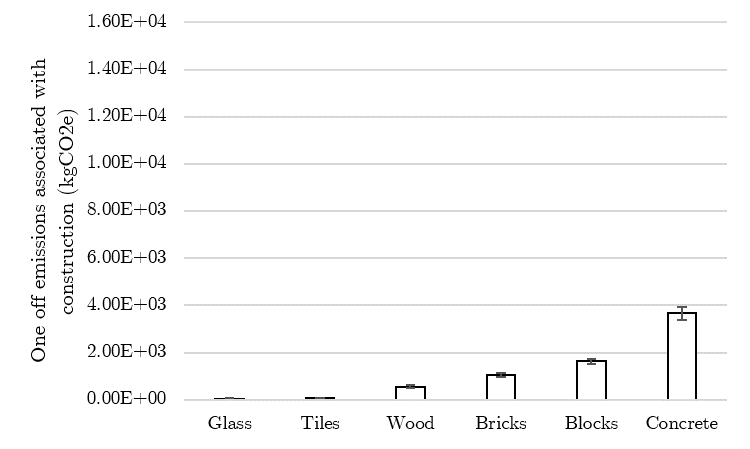
\includegraphics[width=0.45\textwidth]{Figures/Studio.png}
        }
    \subcaptionbox{New build one-bedroom flat}{
    	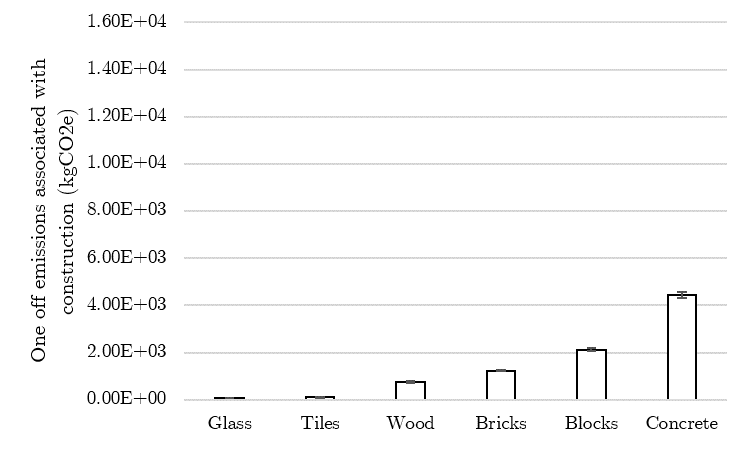
\includegraphics[width=0.45\textwidth]{Figures/1_bed.png}
        }
    \subcaptionbox{New build two-bedroom flat}{
    	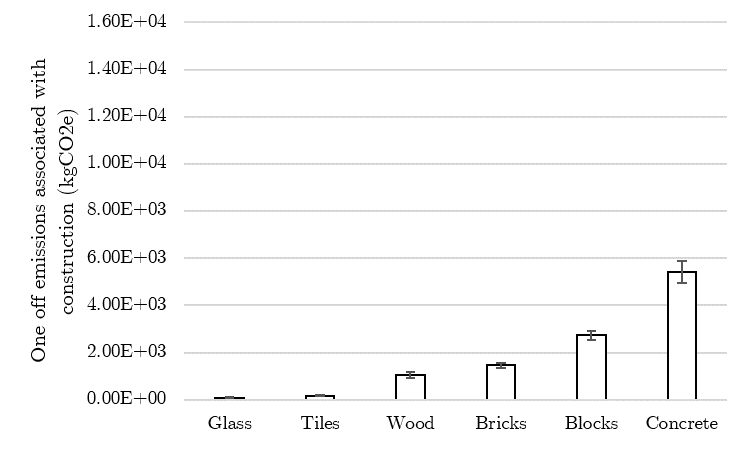
\includegraphics[width=0.45\textwidth]{Figures/2_bed.png}
        }
    \subcaptionbox{New build three-bedroom flat}{
    	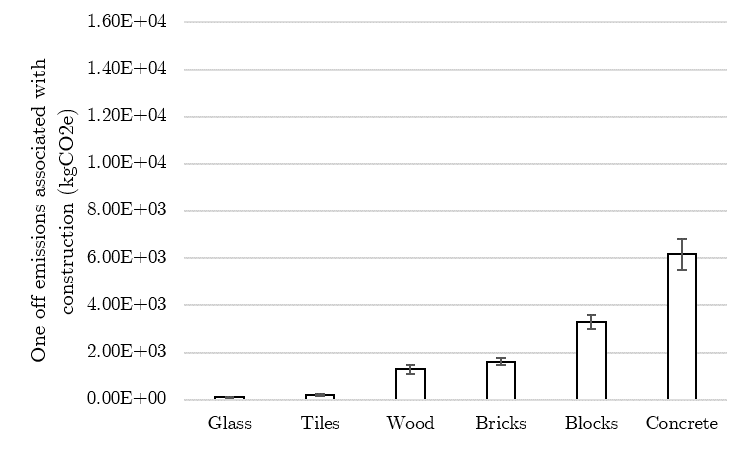
\includegraphics[width=0.45\textwidth]{Figures/3_bed.png}
        }
    \subcaptionbox{New build four-bedroom flat}{
    	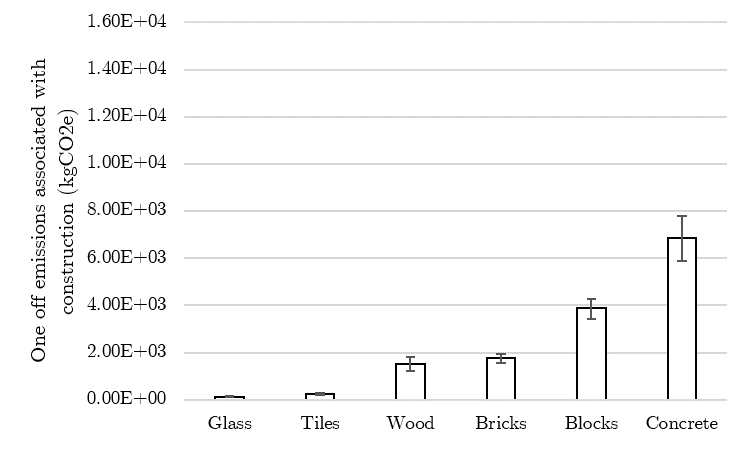
\includegraphics[width=0.45\textwidth]{Figures/4_bed.png}
        }
    \subcaptionbox{New build two storey house}{
    	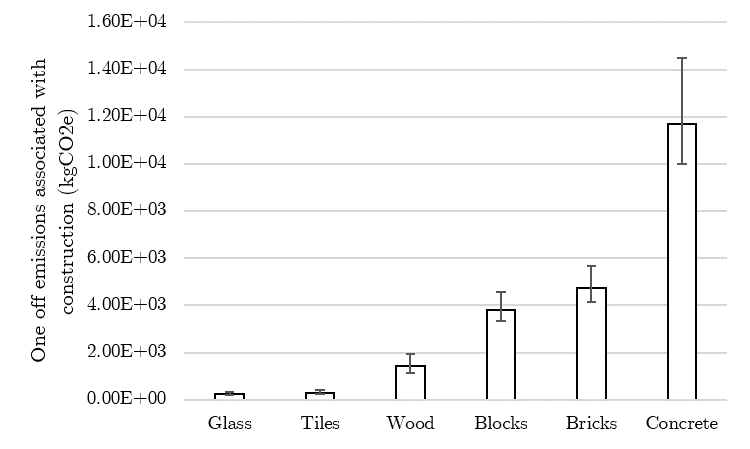
\includegraphics[width=0.45\textwidth]{Figures/2_storey_new.png}
        }
    \subcaptionbox{New build three storey house}{
    	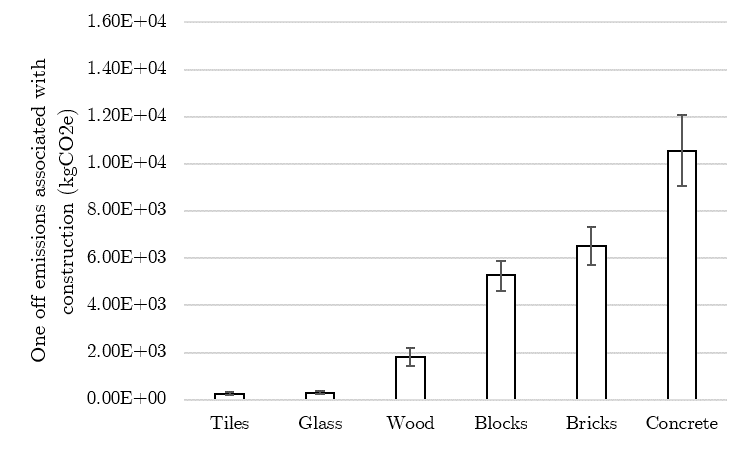
\includegraphics[width=0.45\textwidth]{Figures/3_storey_new.png}
        }   
    \subcaptionbox{One storey extension}{
    	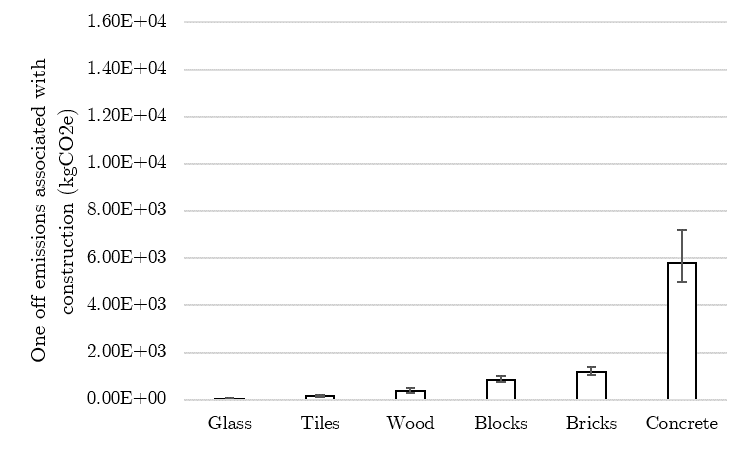
\includegraphics[width=0.45\textwidth]{Figures/1_storey_ext.png}
        }
    \caption{Embodied emissions associated with the as built material requirements of different construction works, calculated using the BOM models developed as in Section \ref{methods}}
\end{figure}
\clearpage
\begin{figure}[!ht]\ContinuedFloat
    \centering
    \subcaptionbox{Two storey extension}{
    	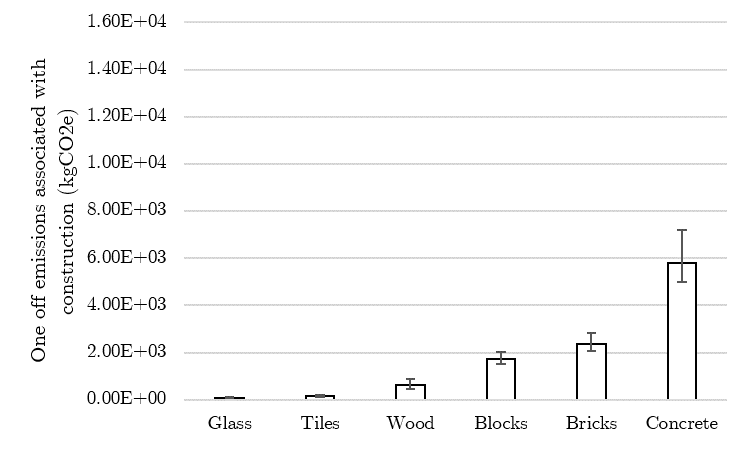
\includegraphics[width=0.45\textwidth]{Figures/2_storey_ext.png}
        }
    \subcaptionbox{Three storey extension}{
    	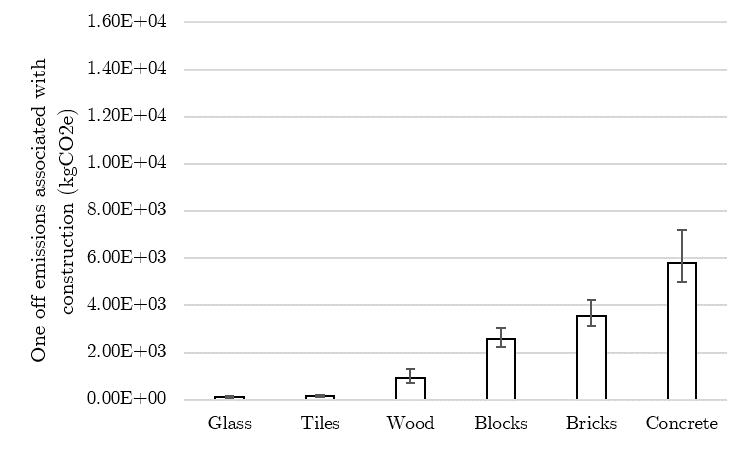
\includegraphics[width=0.45\textwidth]{Figures/3_storey_ext.png}
        }
    \subcaptionbox{Single garage}{
    	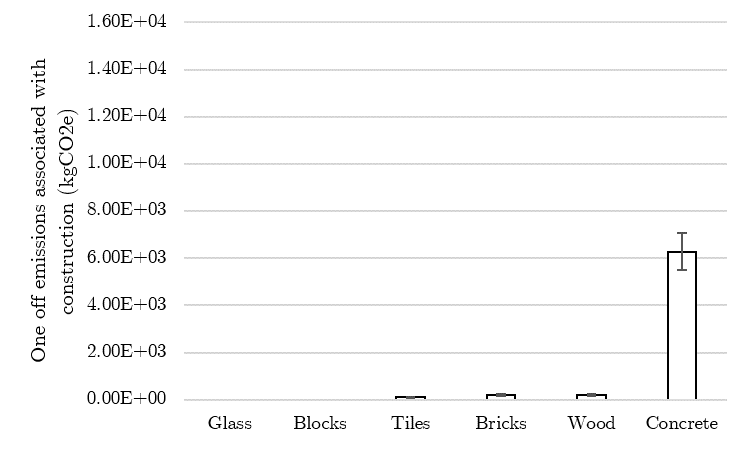
\includegraphics[width=0.45\textwidth]{Figures/Garage_sing.png}
        }   
    \subcaptionbox{Double garage}{
    	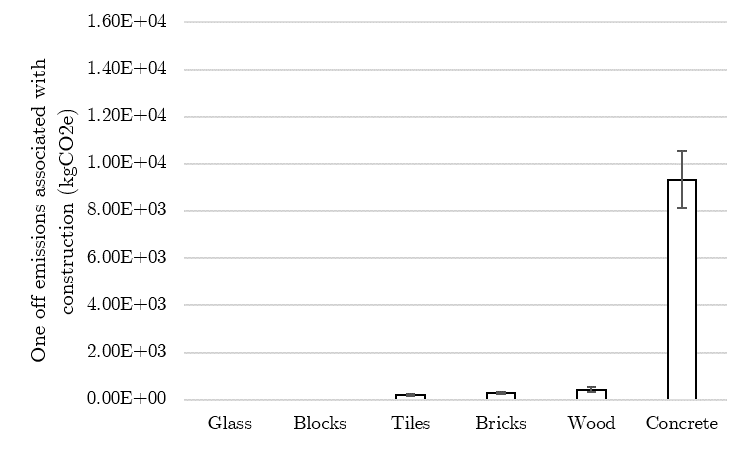
\includegraphics[width=0.45\textwidth]{Figures/Garage_doub.png}
        }   
    \subcaptionbox{Triple garage}{
    	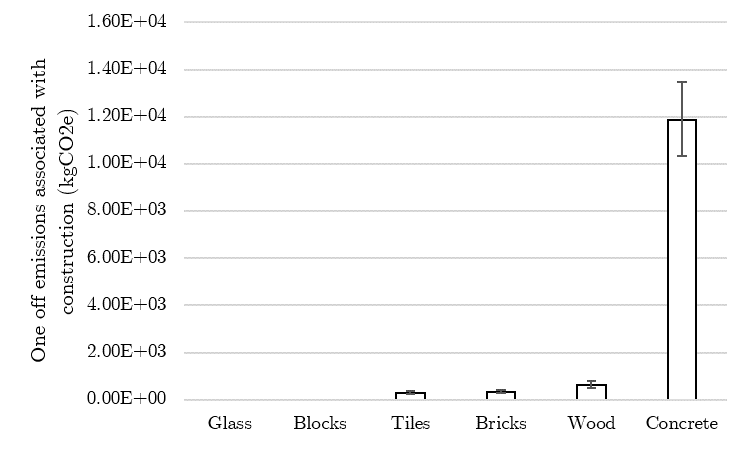
\includegraphics[width=0.45\textwidth]{Figures/Garage_trip.png}
        }   
    \subcaptionbox{Conservatory}{
    	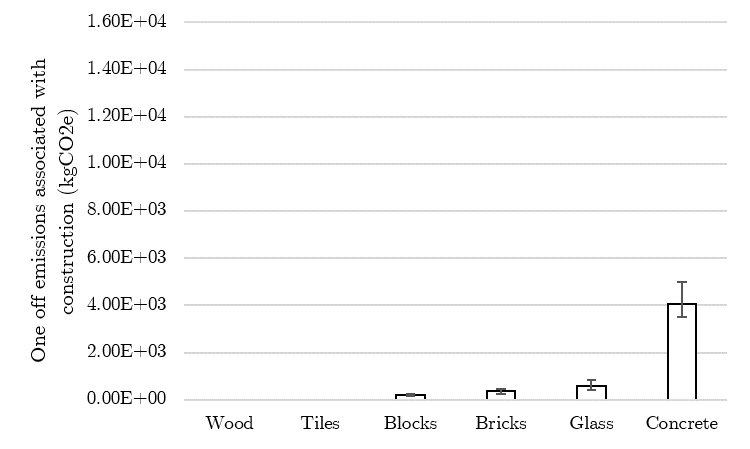
\includegraphics[width=0.45\textwidth]{Figures/Conservatory.png}
        }
    \subcaptionbox{Garden room}{
    	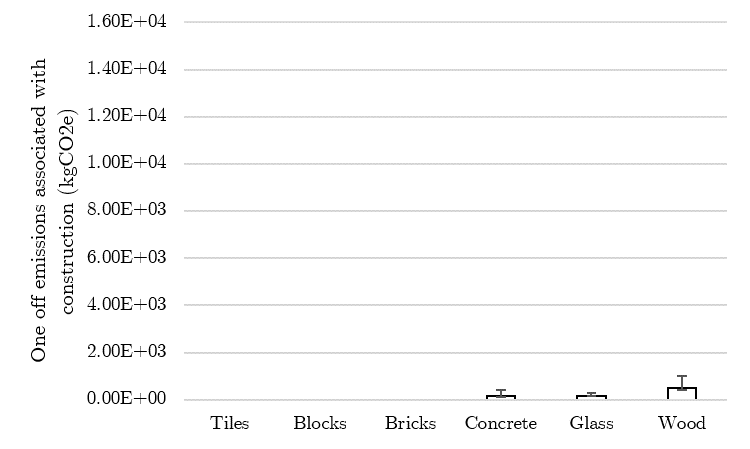
\includegraphics[width=0.45\textwidth]{Figures/Garden_room.png}
        }   
    \caption[]{One off embodied emissions associated with the as built material requirements of different construction works, calculated using the BOM models developed as in Section \ref{methods}}
    \label{fig:individualworksnew}
\end{figure}
\clearpage

\paragraph{}
The annual emissions impact of refurbishing one, two, and three storey dwellings is shown in Figure \ref{fig:individualworksref}. It should be noted that the values seen in this figure are one tenth of the size of those seen in Figure \ref{fig:individualworksnew}.

\begin{figure}[!ht]
    \centering
    \subcaptionbox{One storey refurbishment}{
    	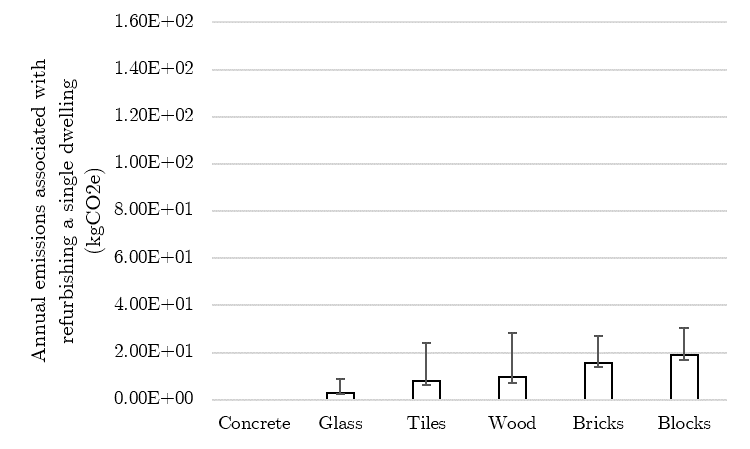
\includegraphics[width=0.45\textwidth]{Figures/1_storey_ref.png}
        }
    \subcaptionbox{Two storey refurbishment}{
    	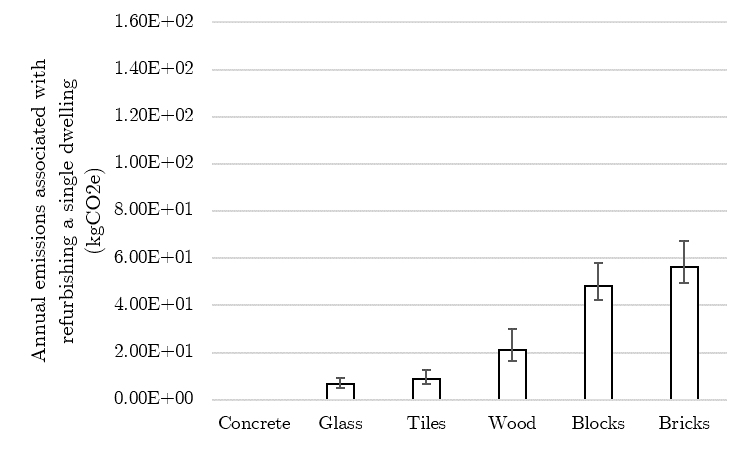
\includegraphics[width=0.45\textwidth]{Figures/2_storey_ref.png}
        }   
    \subcaptionbox{Three storey refurbishment}{
    	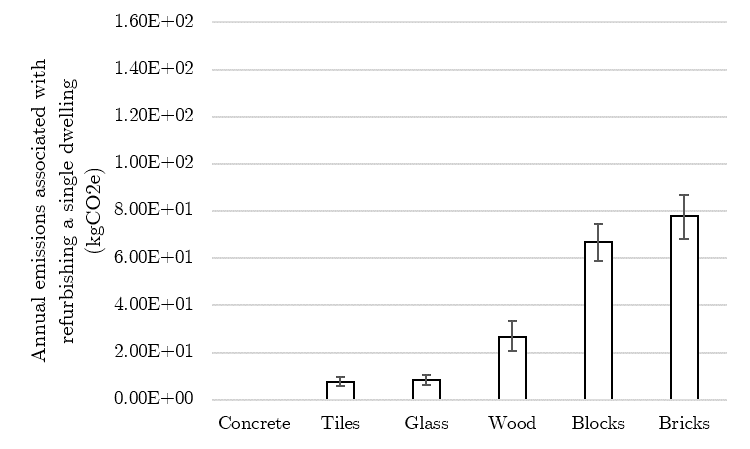
\includegraphics[width=0.45\textwidth]{Figures/3_storey_ref.png}
        }   
        \caption{Embodied emissions associated with the annual material requirements of refurbishing a single dwelling, calculated using the BOM models developed as in Section \ref{methods}}
        \label{fig:individualworksref}
\end{figure}

\paragraph{}
Comparing the total emissions of each type of new construction work, as in Figure \ref{fig:workssummary} shows that new build three-storey houses are the most emissions intensive, followed by two-storey houses and four-bedroom flats.

\begin{figure}[ht!]
    \centering
    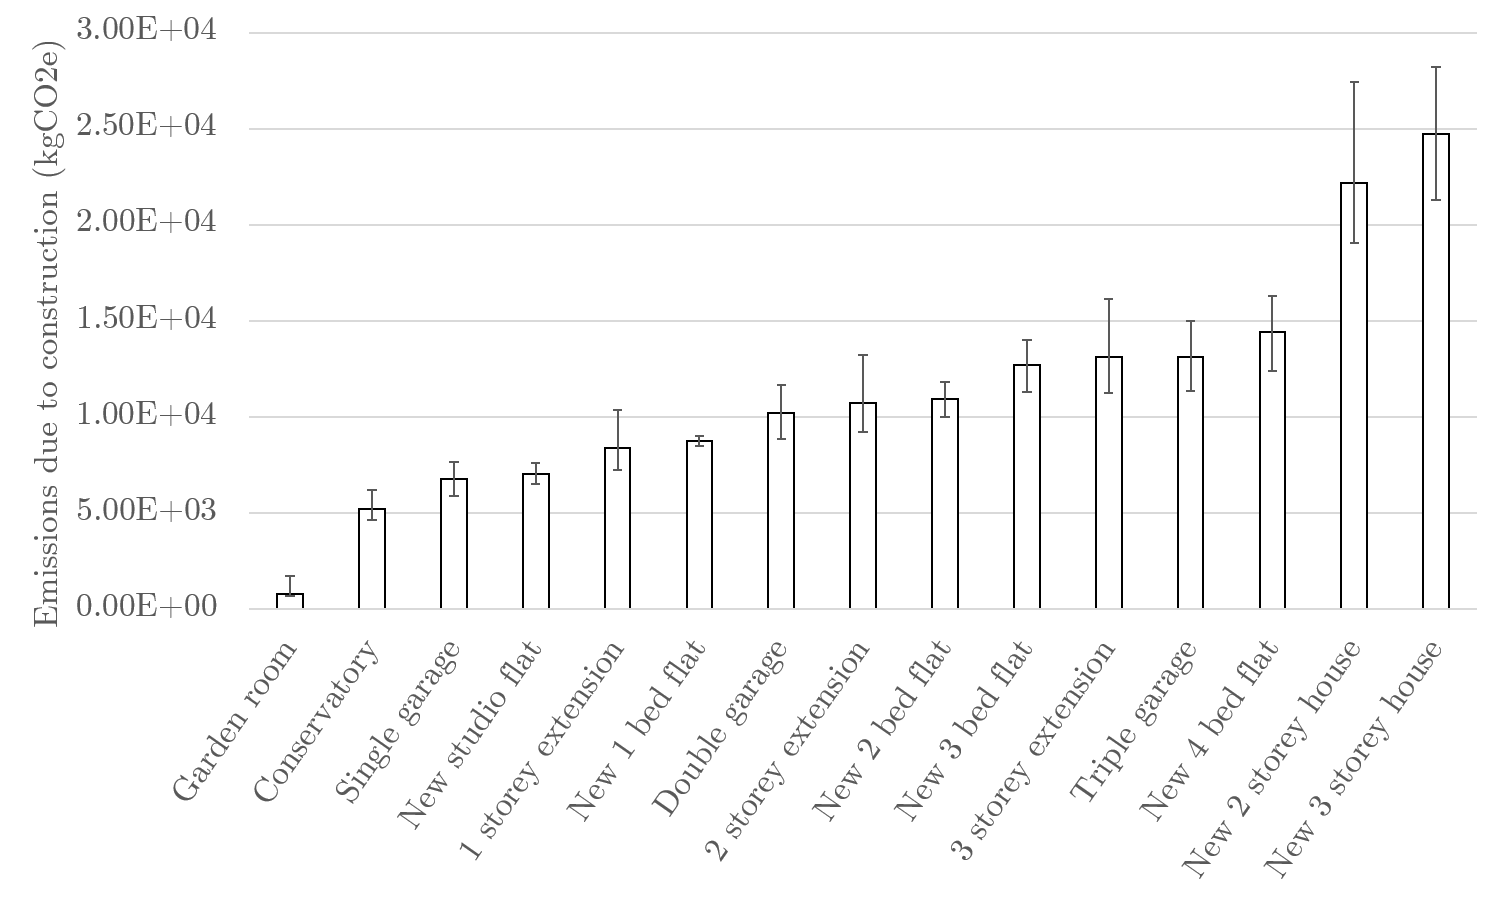
\includegraphics[width=0.85\textwidth]{Figures/Ind_works.png}
    \caption{A comparison of the one-off emissions impact of performing each relevant construction work}
    \label{fig:workssummary}
\end{figure}

\paragraph{}
In a similar way, the emissions associated with the annual refurbishment of different individual dwellings can be compared as in Figure \ref{fig:refurbcomp}.

\begin{figure}[!ht]
    \centering
    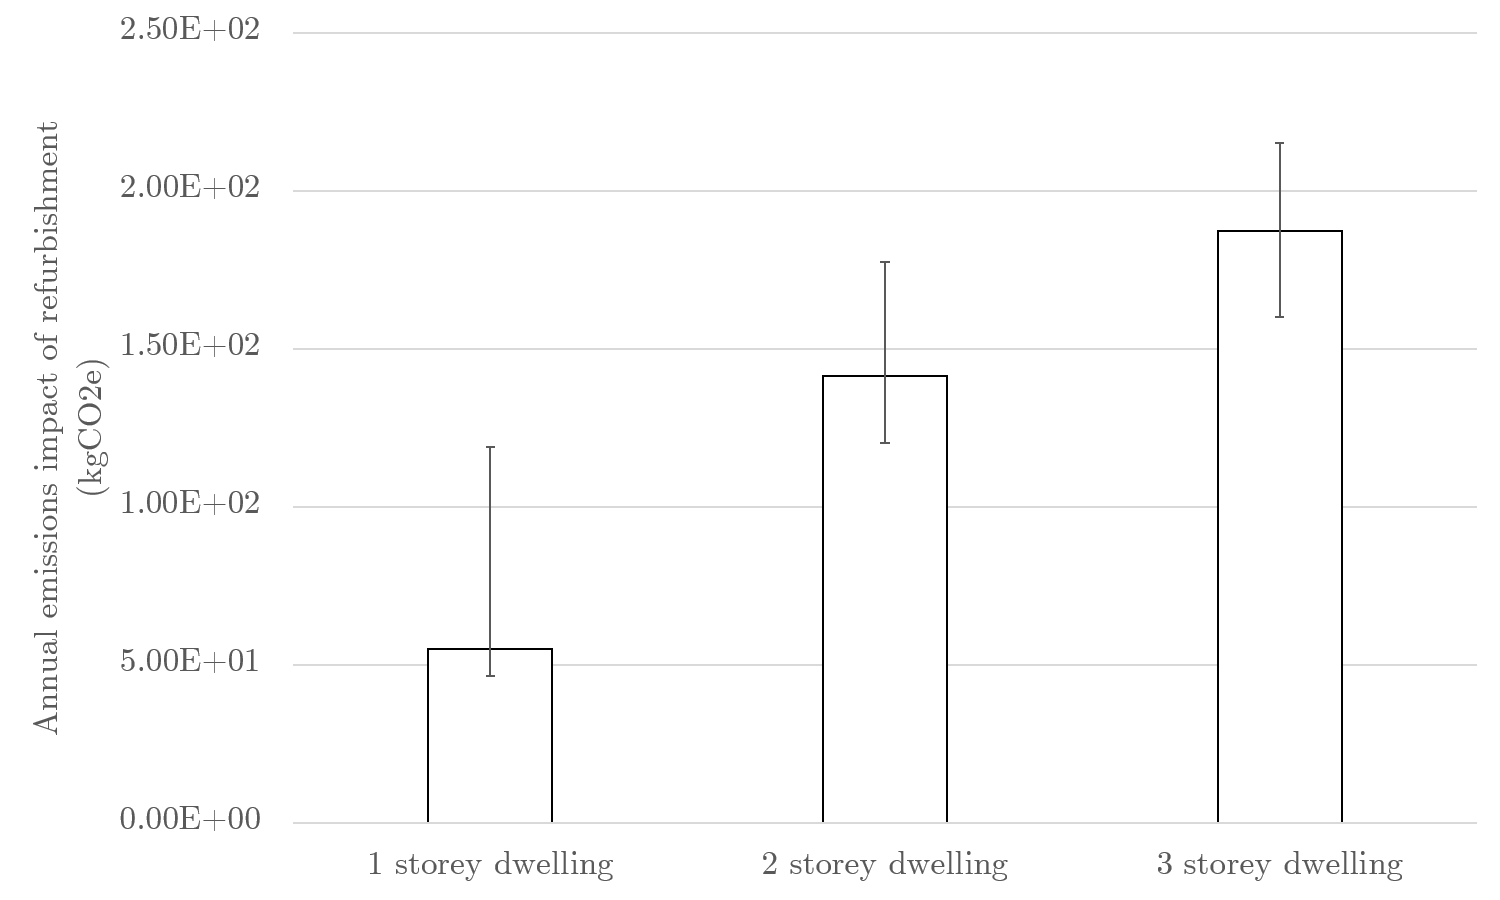
\includegraphics[width=0.85\textwidth]{Figures/Ind_refurb.png}
    \caption{A comparison of the annual emissions impact of refurbishing different dwelling types}
    \label{fig:refurbcomp}
\end{figure}

\paragraph{}
In addition to the profile of individual works, it is possible to derive values for the English stock as a whole. The emissions associated with the annual material requirement of the English housing stock is 8 MtCO\textsubscript{2}e. Figure \ref{fig:emissionsbywork} shows the annual emissions associated with each type of construction work in England. 

\begin{figure}[!ht]
    \centering
    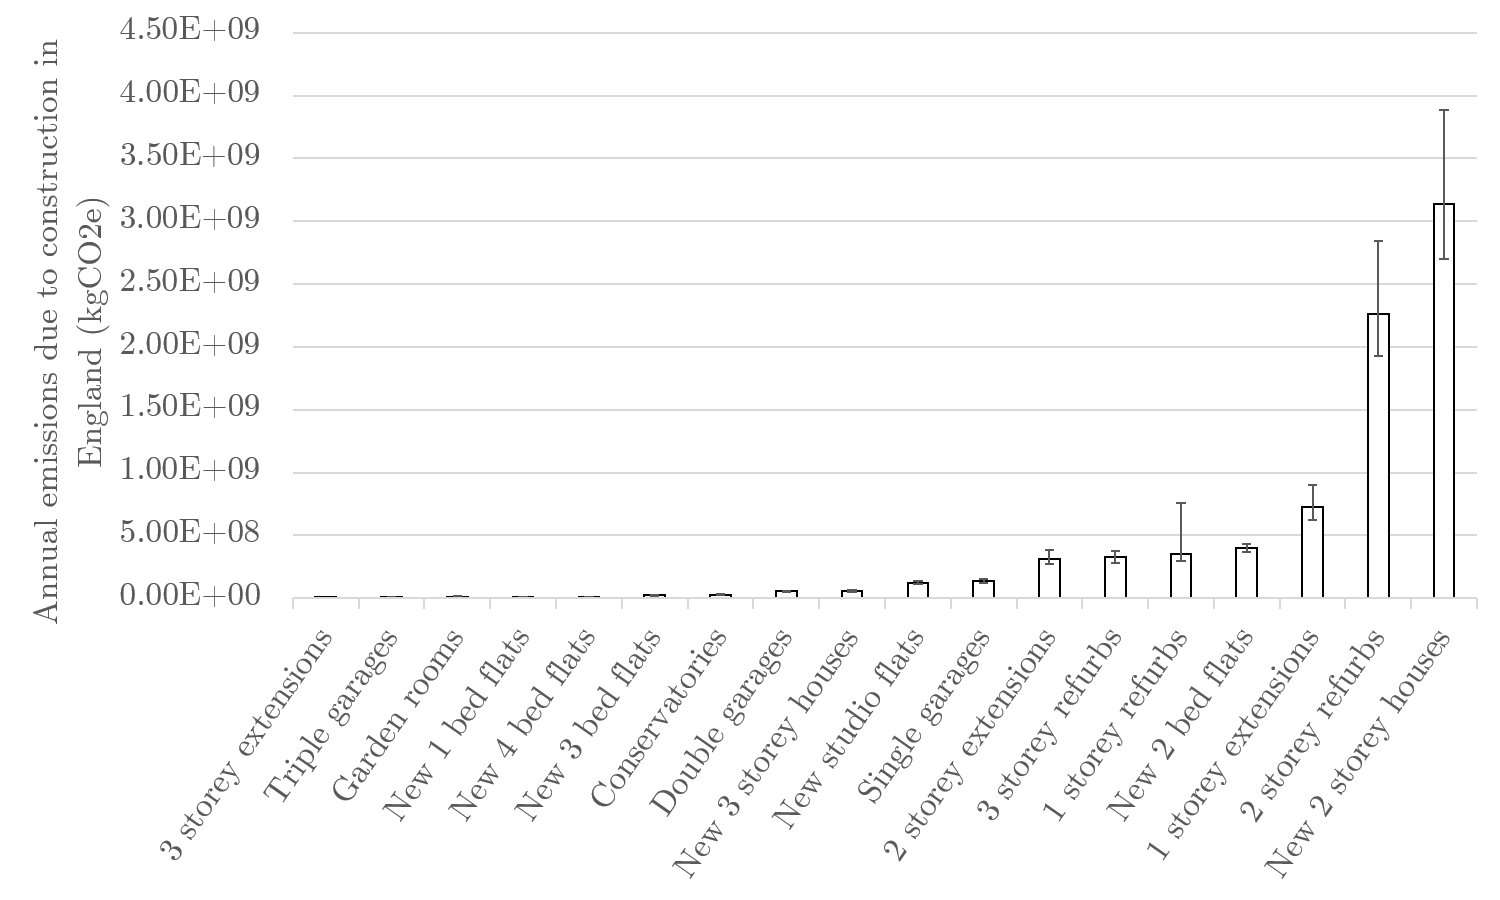
\includegraphics[width=0.85\textwidth]{Figures/Works_eng.png}
    \caption{The annual emissions associated with all the new construction of each different work in England}
    \label{fig:emissionsbywork}
\end{figure}

\paragraph{}
From the underlying data, it can be shown that refurbishments are responsible for 37\% of all emissions. It can also be seen that the new and old two storey houses are responsible for 65\% of annual emissions, through initial material requirements for new builds and refurbishment for existing dwellings. The split between new builds, other additions (extensions, conservatories etc.) and refurbishment is shown in Figure \ref{fig:propssumm}.

\begin{figure}[!ht]
    \centering
    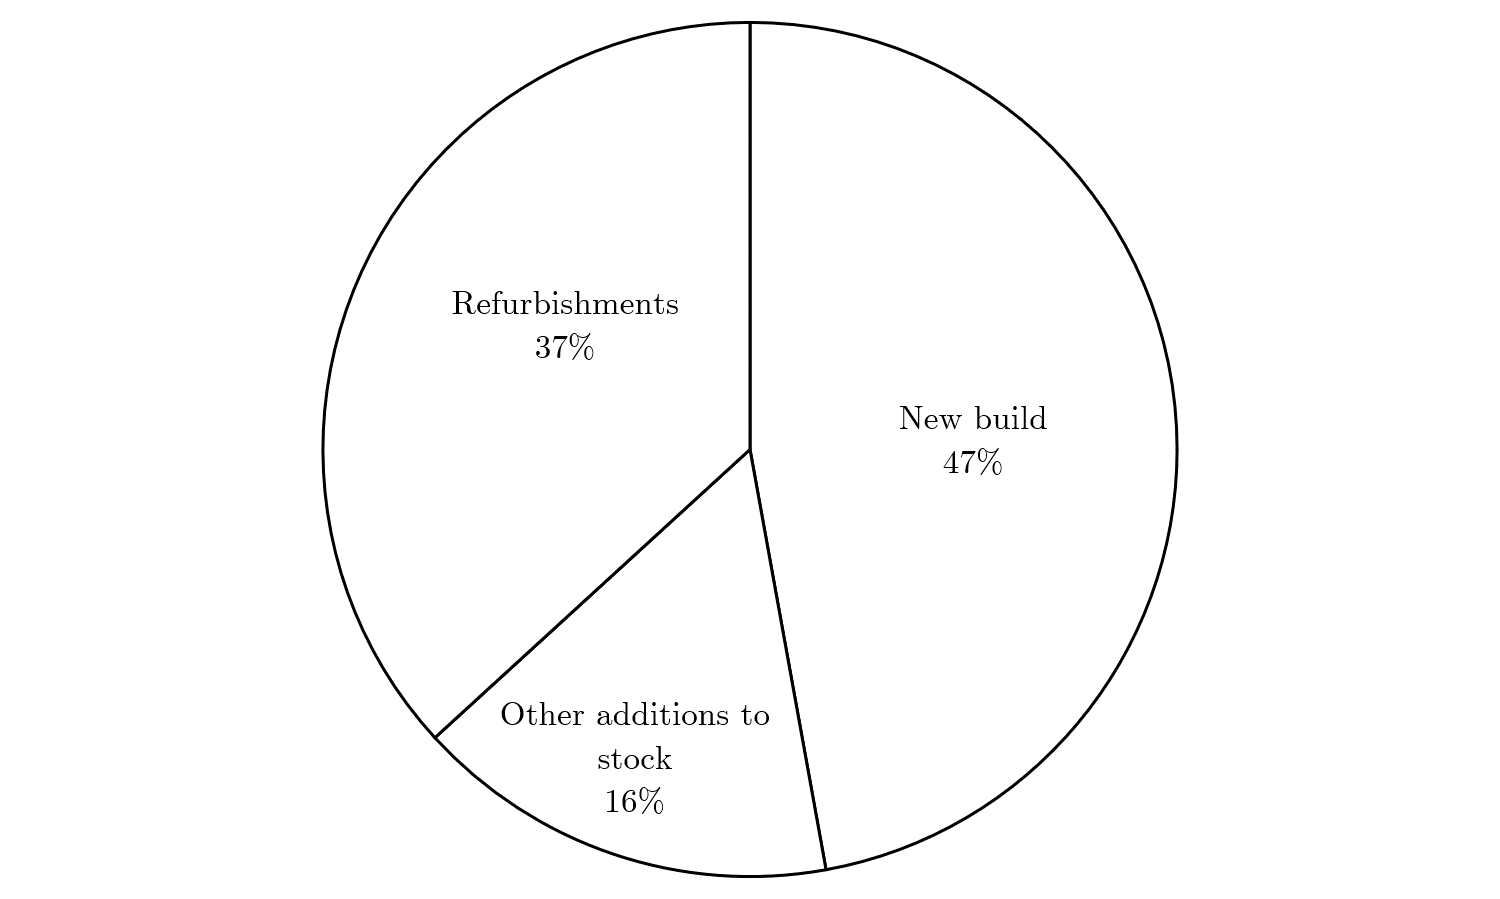
\includegraphics[width=0.85\textwidth]{Figures/Props_summ.png}
    \caption{The proportion of carbon emissions contributed by different types of construction in the residential sector}
    \label{fig:propssumm}
\end{figure}

\paragraph{}
When considering the impact from a material point of view, the results are as shown in Figure \ref{fig:emissionsbymaterial}. From this figure, it can be seen that the material responsible for most emissions in the residential stock is poured concrete, followed by brick. Poured concrete is responsible for approximately 36\% of emissions, whilst brick accounts for roughly 26\%. If concrete is considered more generally by including the effects of precast blocks and roof tiles, this value rises to 62\%. Thus, bricks and concrete contribute close to 90\% of total emissions.

\begin{figure}[ht!]
    \centering
    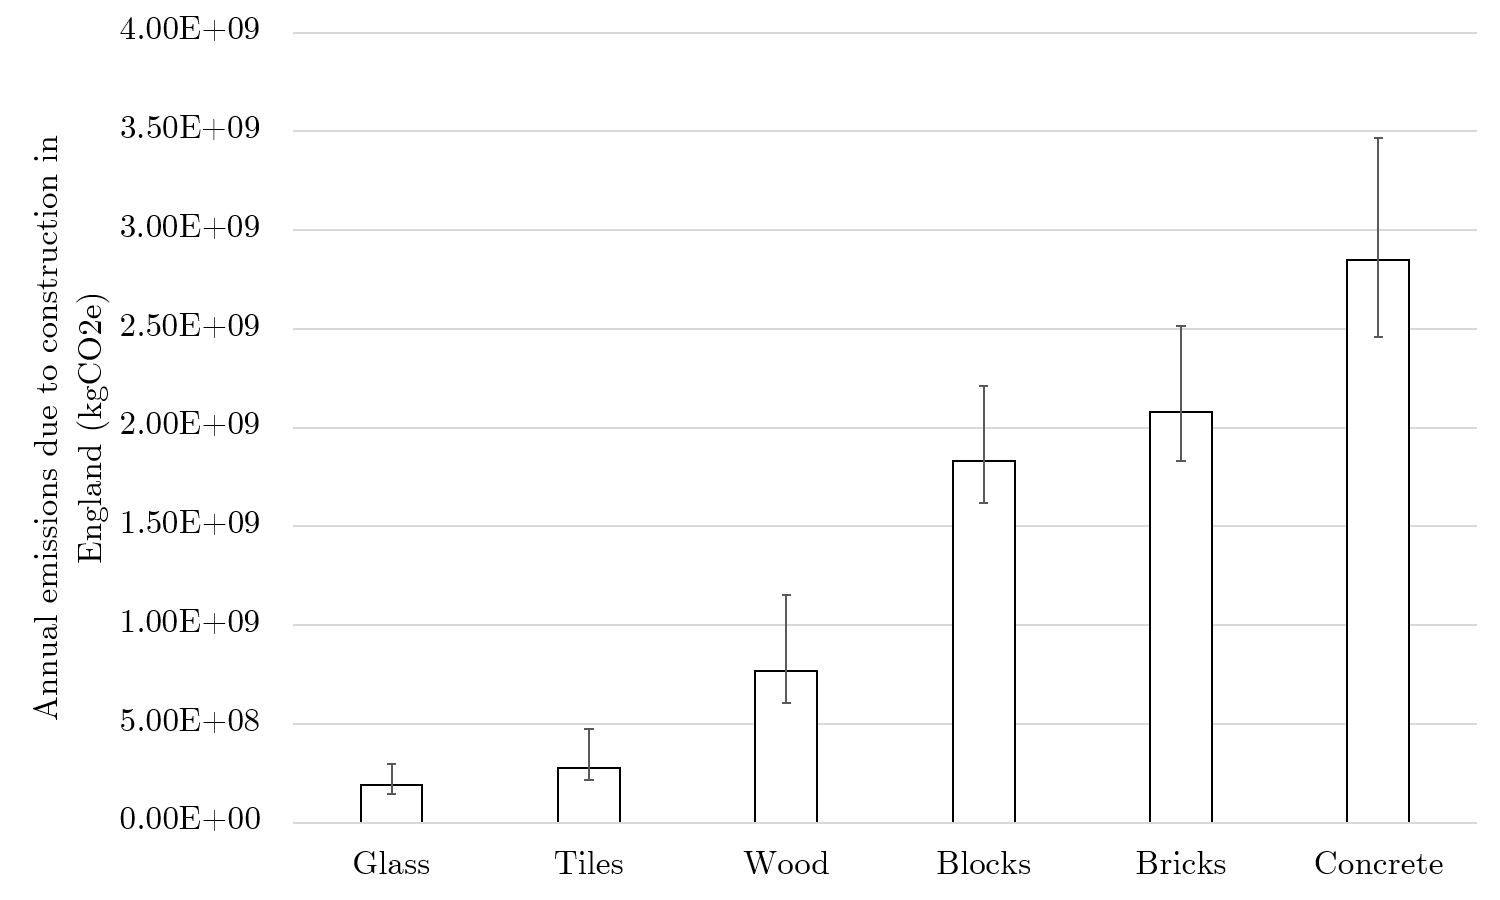
\includegraphics[width=0.85\textwidth]{Figures/Materials_eng.png}
    \caption{The annual emissions associated with each material used in residential construction in England}
    \label{fig:emissionsbymaterial}
\end{figure}

%---------------------------------------
% Discussion
%---------------------------------------

\section{Discussion}
\label{discussion}

\subsection{Placing the results into context}
\label{widercontext}

\paragraph{}
The main aim of this study was to quantify the emissions associated with the annual  requirements of the English housing stock. The equivalent carbon dioxide emissions associated with this is shown to be 8 MtCO\textsubscript{2}e. In 2016, UK net carbon dioxide emissions were estimated to be 374.1 MtCO\textsubscript{2}e \citep{Department_for_Business_Energy_and_Industrial_Strategy2017-oa}. Since 2016 was the year being modelled in this case, the results suggest that the annual material requirement of the English housing stock accounts for around 2.1\% of all emissions. In the same year, total emissions from the residential sector were estimated at 63.4 MtCO\textsubscript{2}e and hence the material input accounts for 13\% of this. 

\paragraph{}
As a quantity previously not well understood, a 2.1\% contribution to UK emissions seems too large a fraction to ignore. It must also be noted that the emissions predictions derived in this report are for the English housing stock, and hence the contribution of the UK stock will be a higher proportion of total emissions. By comparing the residential stock in England with the residential stock in the UK, it can be crudely estimated that in fact the material requirements of housing contribute closer to 3\% of carbon dioxide emissions. Comparing with statistics published by the \citet{Department_for_Business_Energy_and_Industrial_Strategy2017-oa}, the value derived in this report is almost twice the emissions contributed by agriculture and comparable to the contributions of both the public sector and industrial processes.

\paragraph{}
As a larger contributor than entire sectors with well described policy in place, it is clear that the UK lies behind the curve with regards to reducing emissions from material input to the residential stock. Whilst the relative focus on in-use emissions may be justified, there is certainly worth in considering efficiency measures with regards to embodied emissions since any consequential emissions savings would not be negligible.

\paragraph{}
It is also unexpected to see the emissions impact of refurbishment to be comparable to that of new builds. Refurbishment of the existing housing stock is estimated to account for 37\% of embodied carbon emissions in an average year. With a decreasing rate of demolition and continued stock growth, it follows that the contribution of refurbishment to the emissions associated with the housing stock is likely to increase. At a time when the UK is not on track to meet carbon budgets, a shift in focus will be required to try to reverse this trend. Emissions reduction potential is largely two-fold; either a reduced demand for residential construction, or a reduction in the emissions associated with the material demand would ensure emissions savings in the future.

\subsection{Recurrent embodied emissions}

\paragraph{}
As proposed in literature, annual recurrent embodied emissions account for 0.5-0.9\% of initial embodied emissions. The results of this study agree with these estimations, with the annual embodied emissions from refurbishment of one, two, and three storey dwellings estimated at 0.51\%, 0.64\% and 0.76\% of initial embodied emissions respectively. A main contributor to the difference in estimates is the different wall areas involved with each type of dwelling, with bricks having an estimated mean intrinsic service life of 84 years and concrete blocks 79 years. The average service life of a dwelling assumed in literature is 59 years \citep{Dixit2019-bj} - if this were the case in practice then there would be no need for the replacement of bricks or blocks at all. Since only around 10,000 dwellings are classified as being demolished each year, it seems unlikely that all houses only survive 59 years \citep{Ministry_of_Housing_Communities2012-zw}. Clearly there is a relevant question regarding the point at which large-scale refurbishment becomes demolition and rebuild, but with so few demolitions being reported, it seems realistic that bricks and blocks be considered as part of refurbishment works.

\paragraph{}
The method presented in Section \ref{methods} also assumed refurbishment to begin at the same time a new build is completed. Again, in practice this is not the case. When averaged over a long time-frame however, it does correctly describe the situation for a large proportion of English housing, since the majority of the stock is made up of dwellings older than the service life of many of their component parts.

\paragraph{}
Whilst refurbishment accounts for less than one percent of initial embodied emissions annually for each individual dwelling, when analysing the stock as a whole, refurbishment plays a much larger role; refurbishment accounts for 37\% of all embodied emissions. This is due to the rate of additions to the stock being relatively low in comparison with the size of the stock. The absolute value of refurbishment emissions is also increasing as the stock grows at roughly 1-2\% a year and is likely to increase into the future as the Government attempts to deal with the current housing shortage.

\subsection{Emissions segmented by works}

\paragraph{}
Identifying two storey houses as responsible for 68\% of residential embodied emissions could be surprising, however it is less so when considering that 80\% of houses within the stock have two storeys \citep{Department_for_Communities_and_Local_Government2010-op}. In exploring the emissions from houses in particular, a comparison of the estimated emissions obtained in this report with those seen in previous literature yields some agreement. \citet{Suzuki1995-ve} reported estimates of the embodied emissions intensity of residential housing as 250-850 kgCO\textsubscript{2}e/m\textsuperscript{2} - in this study the values are estimated as 150-260 kgCO\textsubscript{2}e/m\textsuperscript{2}, as shown in Figure \ref{fig:bym2}. 

\begin{figure}[!ht]
    \centering
    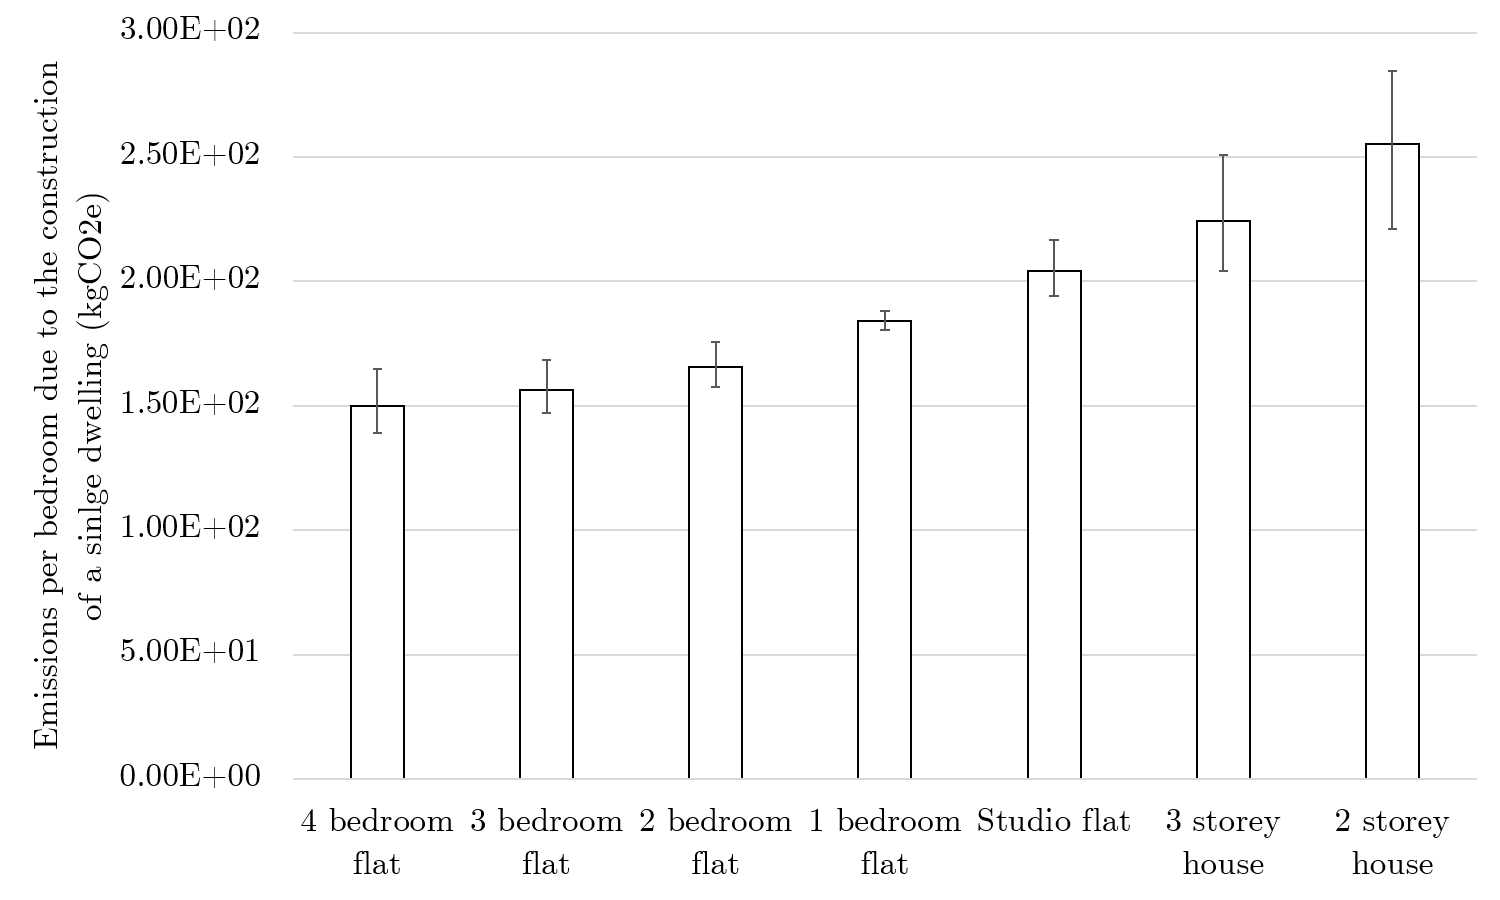
\includegraphics[width=0.85\textwidth]{Figures/Per_m2.png}
    \caption{A comparison of the emissions per square meter of floor area associated with new build housing in England}
    \label{fig:bym2}
\end{figure}

\paragraph{}
The values predicted by \citet{Suzuki1995-ve} were the result of studying three different types of houses, all of which had two or more storeys. Different construction methods were also considered, explaining the wide range of values proposed. When exploring the values derived in this report, the most relevant comparison to make is one between two storey houses. \citet{Suzuki1995-ve} predict the emissions intensity of two storey housing to be between 250 and 450 kgCO\textsubscript{2}e/m\textsuperscript{2}. This report predicts a value of 260 kgCO\textsubscript{2}e/m\textsuperscript{2} - within the bounds but at the very low end. This is unsurprising given that the model used in this case does not encompass all materials used in residential construction. The smaller variation in results from this investigation, when compared with those in literature, is likely a function of the simplifications made with regards to materials and construction methods used.

\paragraph{}
Whilst the results seen in previous literature and found here do agree somewhat, it does not necessarily provide justification for the scaling of individual case studies. The extrapolation of single cases may still lead to large inaccuracies in the estimation of quantities of materials used and hence introduce error into any further calculations. For example, the majority of life cycle analyses described in Section \ref{PreviousLiterature} are for two storey family houses. Extrapolating results from these would ignore the presence of different dwelling types within the stock and, as this study has shown, each dwelling type contributes a different amount of embodied emissions. This is not to say that the estimation of materials here is entirely correct, just that the problem has been considered with extrapolation in mind. Hence, assumptions have been made with the explicit intention of being representative of the stock as a whole, in a way that would not be true for many case studies.

\paragraph{}
That all dwelling types seem to result in similar emissions densities is an important result in itself. As such, there is no single stand-out candidate for emissions reductions when it comes to material requirements and hence widely targeted policies would be required in order to reduce embodied emissions. As expected, larger dwellings have a lower emissions density than smaller ones due to material input not being a linear function of floor area. Two storey houses have the highest emissions density, followed closely by studio flats. The least emissions dense dwelling type modelled in this study is four-bedroom flats and hence would be an emissions efficient way of expanding the housing stock. At the current time, four-bedroom flats account for less than 0.5\% of dwellings in England \citep{Ministry_of_Housing_Communities2012-ez}. 

\paragraph{}
When considered as embodied emissions per bedroom, the dwellings that perform the worst are one-bedroom flats, although studio flats and two storey houses are again high on the list. This is displayed in Figure \ref{fig:bybedroom}, which allows all dwelling types to be compared. It would therefore seem as though moving from small self-contained units to larger shared dwellings would be one way of reducing embodied emissions in the long term since this would also reduce the absolute demand for new dwellings. This is obviously not a viable solution since we cannot feasibly force citizens to live in shared dwellings. It could, however, be a beneficial policy to focus on ensuring existing space is filled such that demand for new builds might decrease in the future.

\begin{figure}[!ht]
    \centering
    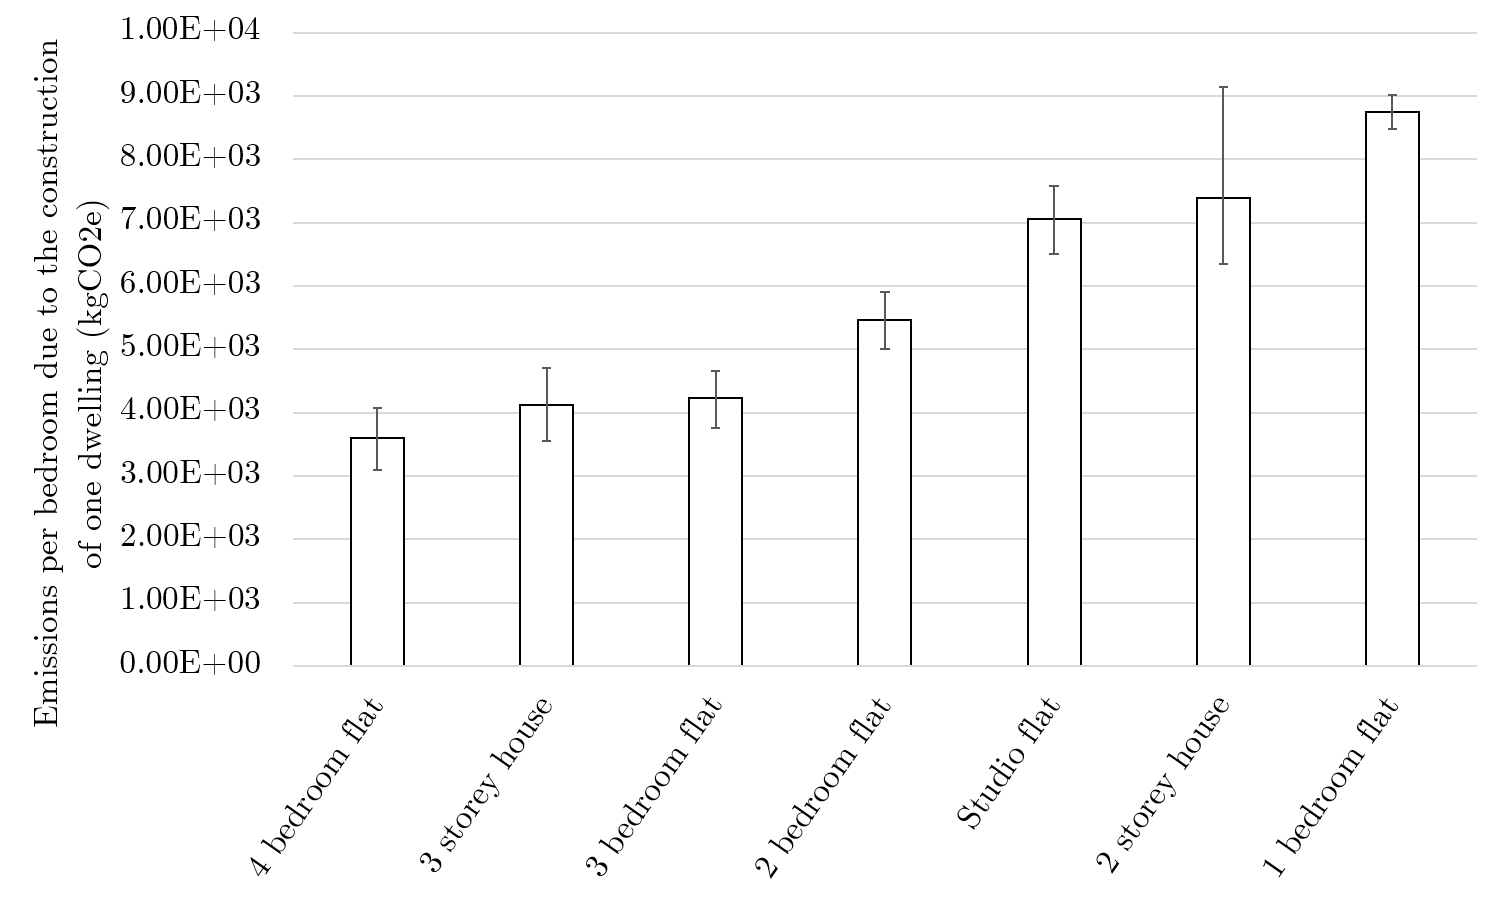
\includegraphics[width=0.85\textwidth]{Figures/Per_bedroom.png}
    \caption{A comparison of the emissions per bedroom associated with new build housing in England}
    \label{fig:bybedroom}
\end{figure}

\subsection{Emissions segmented by materials}

\paragraph{}
By considering only six key materials and only one basic housing design, it is true that quantities of certain materials have been ignored. This is likely to go some way to explaining why the values estimated by \citet{Suzuki1995-ve} are higher than those predicted here. The drop off in emissions seen in Figure \ref{fig:emissionsbymaterial}, however, is consistent with the assumption that the materials used in smaller quantities can be reasonably neglected when producing a high-level estimate for the stock as a whole.

\paragraph{}
The Government publishes quarterly statistics on building materials and components in the UK \citep{Department_for_Business_Energy_Industrial_Strategy2019-va}. These can give more context to the results derived in this report and, whilst the two estimates are not expected to match up exactly, due to the major simplifications made in the methods here, they might give some indication as to the reliability of the model. In quantifying the total concrete usage in the English housing stock, poured concrete, precast blocks, and roof tiles can all be combined to give an estimate of the overall volume of concrete used. This volume can then be used to estimate the mass of sand, gravel and cement involved. \citet{Shanks2019-nu} predicted that 36\% of UK cement use is by the residential sector. The model detailed in this report predicts a cement requirement in England of 2.9 Mt/year and hence 32\% of total usage, a reasonable agreement.

\paragraph{}
Whilst the concrete estimation seems to agree well, the amount of bricks, blocks, and tiles calculated by the same method show slight overestimates. This can be explained by the oversimplification of the stock in assuming that all dwellings are built in the same way. For example, it is not true that all dwellings are built using brick and block cavity walls, nor do all dwellings use concrete roof tiles. This is unlikely to have a significant impact on the associated emissions, however, since any houses not constructed using brick would still be constructed using similar amounts of another material, often of comparable embodied carbon. For example, in replacing the volume of bricks used with an equivalent volume of timber, the total annual embodied emissions are changed by less than 1\% - far smaller than the errors quoted for values derived in this report.

\paragraph{}
A study by \citet{Lawania2016-er} on which type of building envelope leads to the lowest life cycle emissions in a typical house concluded that forty envelope options existed that provided lower life cycle emissions than the conventional brick envelope. Whilst a complete move away from bricks does not seem feasible, encouraging house builders and homeowners to use more energy efficient materials could help to reduce the emissions associated with residential construction. There is an indication that this change is already taking place, with the total brick production in the UK falling by 20\% between 2011 and 2015 when normalised by the total number of new dwellings built each year \citep{Ministry_of_Housing_Communities2012-zw,Department_for_Business_Energy_Industrial_Strategy2019-va}. 

\paragraph{}
A report by the \citet{National_Audit_Office2005-mw} noted that brick and block construction was the most time intensive but also the cheapest of all construction techniques compared. This suggests that the house building industry is primarily cost-driven, rather than time driven and hence this must be addressed if a real impact is to be made on the amount of bricks used. The cost of more modern construction methods must be reduced in order to make them attractive to consumers and provide some incentive to owners to request homes of lower embodied emissions.

\paragraph{}
Whilst brick is a large contributor to emissions from residential construction, concrete remains the area of focus, just as it is in commercial construction. \citet{Gagg2014-nc} notes that concrete is the second-most used material in the world after water and hence emissions savings measures would have a wide-scale impact. Since an alternate material with sufficient mechanical properties, as well as being cheap, does not appear to be forthcoming it is unlikely that the demand for concrete as a construction will fade in the near future. A focus on reducing both the amount of concrete used and the emissions associated with concrete manufacture would therefore go a long way to reducing the embodied emissions in the residential stock. Reducing absolute demand for concrete, in particular, would result in significant emissions savings; \citet{Shanks2019-nu} estimated that cement demand could be reduced by 51.3\% through more efficient material use. 

\subsection{Sensitivity of emissions estimation to temporal effects}

\paragraph{}
The estimation made in this study assumes a single construction method with common construction materials and is based on data from 2016. It is therefore true that conclusions drawn from this data may not apply so well to different years and different geographies. Two of the main effects of considering different time periods would be to change the size of the current stock and number of new builds, and also to change the characteristics with which dwellings are built. 

\paragraph{}
Changing the size of the stock would directly impact the values calculated in this report and hence percentage values are potentially more useful than absolute ones. Expressing the embodied emissions associated with the material requirements of the housing stock as a percentage of total English emissions will allow for comparison over a time frame during which both numbers are likely to change. It also allows progress made in this specific area to be easily bench-marked against that in other sectors and in the country as a whole.

\paragraph{}
Adjustment in construction methods would likely alter the emissions contributions of different materials, although it is not expected that it would have a large effect on total emissions. The \citet{nhbc_2015-cg} reports a general trend in residential construction from solid walls in Victorian times, through brick cavity walls between the wars, to brick and block cavity walls seen now. The effect of the changing construction methods can be modelled by changing the assumptions noted in Section \ref{MaterialReqs}. If it was assumed that the English stock was built with solid brick walls, rather than the most common brick and block cavity design, predicted total embodied emissions would increase 11\%. This change has less of an impact than a 20\% rise in the number of new builds in a given year, something not entirely unlikely when considering three of the four years between 2013 and 2017 saw increases of between 10\% and 20\%. It can also be found that each new design reported by the \citet{nhbc_2015-cg} has increased the insulating properties of dwelling walls, hence contributing to a reduction of in-use emissions over time. 

\paragraph{}
It is therefore clear that the result of the analysis performed in this study is more sensitive to the size and make-up of the housing stock than the construction methods or specific materials used. This provides confidence in the assumption made regarding wall make-up in flats, whereby half of the perimeter walls were assumed to be internal to the development. From this basic sensitivity analysis, it can be shown that that specific assumption has a relatively low impact on the value of total embodied emissions, whilst also providing a reasonable estimation of the true situation. Clearly this only holds true to a certain extent and it would not represent a suitable analysis for a stock involving a full overhaul of construction methods. It is, however, representative enough of the stock in this case to allow meaningful conclusions to be draw. On one hand, this highlights the importance of having good data on the current housing stock, although it also promotes the applicability of the model to other stocks built using similar methods.

\subsection{Effect of results of future policy}

\paragraph{}
As noted in Section \ref{widercontext}, emissions reductions in this area can be achieved by either reducing demand for new materials or by reducing the emissions associated with materials used. Estimates by \citet{Wilson2018-ug} put the number of new homes needed in England at between 240,000 and 340,000 per year. The amount of new homes built annually has been increasing for a number of years however it is still below the amount needed, as shown in Figure \ref{fig:stockadditions} \citep{Ministry_of_Housing_Communities2012-zw, Wilson2018-ug}. The Government, when elected in 2017, set out the target to complete the delivery of one million homes from 2015-2020 and deliver half a million more by the end of 2022. At the same time that many sources doubt whether this target is ambitious enough to meet the needs of society, there is also doubt over whether this number is actually achievable.

\begin{figure}[ht!]
    \centering
    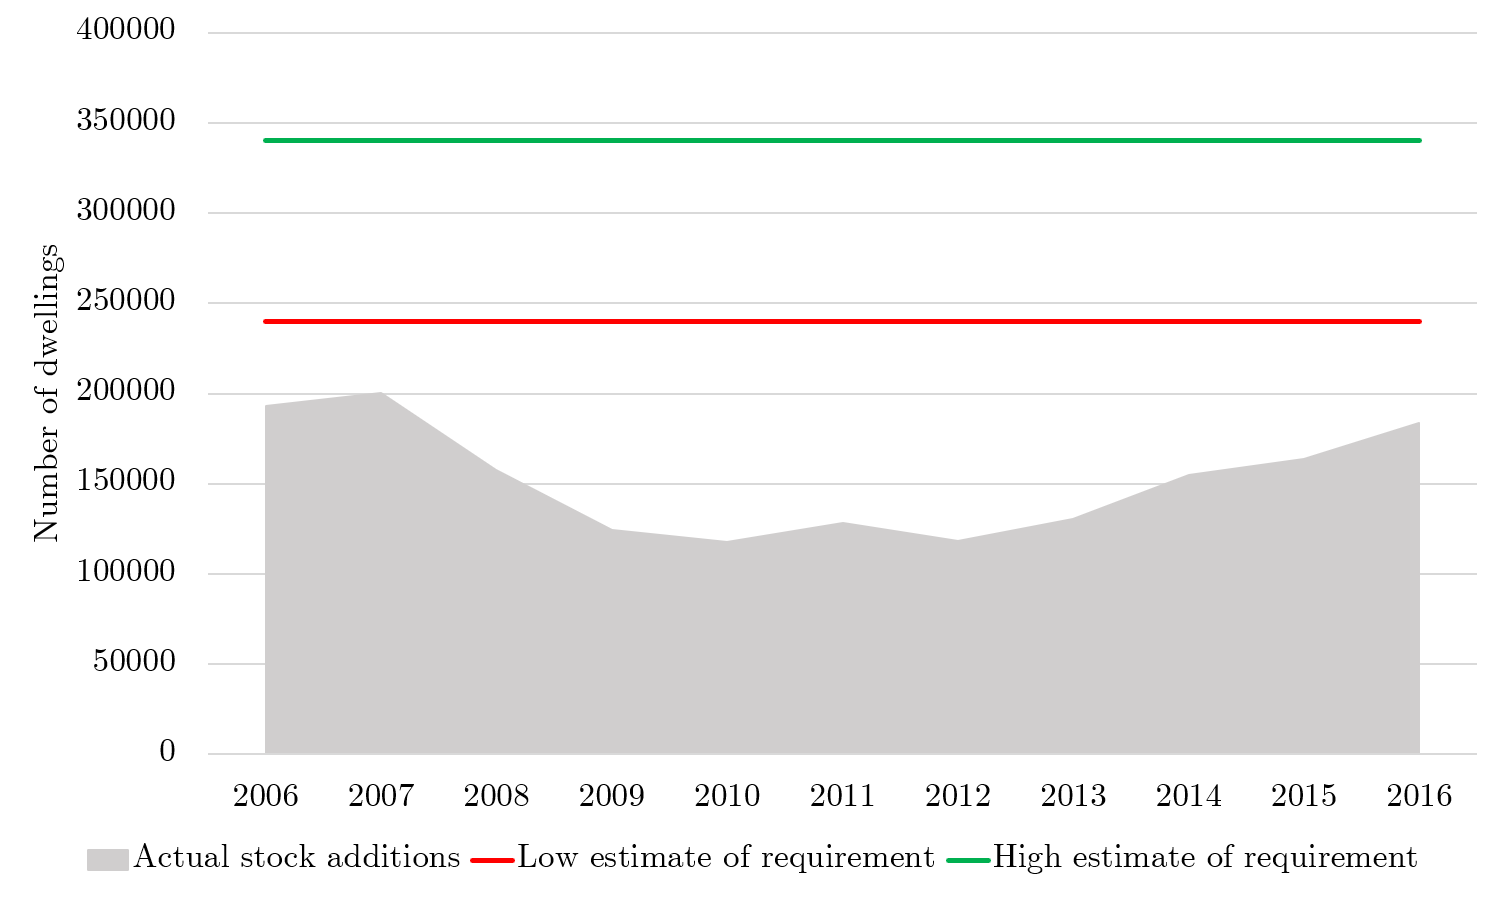
\includegraphics[width=0.85\textwidth]{Figures/Undersupply.png}
    \caption{An illustration of the under supply of housing in England. As first shown in a report by \citet{Wilson2018-ug} but reproduced here}
    \label{fig:stockadditions}
\end{figure}

\paragraph{}
In their 2015 manifestos, all major political parties pledged to increase the rate of additions to the housing stock in order to meet the current shortfall \citep{Wilson2018-ug}. This indicates a widespread consensus that more residential construction is needed and hence reducing the demand for new build homes seems ambitious. There is potential to limit the impact of new construction by encouraging the efficient use of space and re-use of old buildings and their materials when constructing new ones, although emissions reduction efforts should not be simply limited to this.

\paragraph{}
In contrast to reducing demand for residential construction, there is scope to reduce the emissions associated with materials used in the sector. This could be done by manufacturing currently used materials in a less emissions-intensive way, by using a smaller amount of emissions intensive materials, or by switching to greener materials. As noted beforehand, there does seem to be some shift away from traditional construction methods and materials and towards more energy-efficient ones. This should obviously be a considered decision taking into account the full life cycle emissions of a building, although there are solutions which reduce both embodied and operational emissions. 

\paragraph{}
Many materials are already produced with highly optimised processes with limited scope for radical improvement. Some English demand is also now met by overseas supply-chains and hence the opportunity to produce materials in a less material-intensive way is limited. \citet{Giesekam2014-eg} therefore note the importance of reducing overall throughput of these materials through the increased use of alternative materials, methods and technologies. Whilst many alternatives do exist, more exploration is needed to try to characterise and overcome the barriers to greater uptake amongst industry professionals. Further potential solutions could involve changes in recommendations to reduce over-specification of buildings and further education about the benefits of more environmentally aware construction. 

\paragraph{}
Another way to reduce the emissions associated with the materials used in the residential sector would be to increase the rate of re-use and recycling. \citet{Giesekam2014-eg} found that demolition has become increasingly popular relative to deconstruction due to time constraints, health and safety, and financial considerations. Whilst the recycling of construction materials has increased recently, the levels of re-use have declined radically. Motivating an increase in re-use would rely on further consideration of the end-of-life stage in the design of dwellings and hence suitable incentives should exist. Re-using materials would allow lower levels of new material to be produced, hence decreasing the annual emissions associated with the sector.

\subsection{Reliability of the analysis and calculation of error}

\paragraph{}
Throughout the development of the model, data has been drawn from multiple different sources to try to increase reliability. In the cases where this was not possible, sources that expressed ranges of data were used as a preference, such that the level of error involved in calculations could be gauged. All BOM models have associated error, as do the values used to scale up the initial Cambridgeshire analysis. The vast majority of errors, when considering individual materials and each different construction work, lie within ±25\%, although many results are more accurate than that. This is also true of the final estimation of embodied emissions; the final value is subject to a maximum error of -16\% and +27\%, due to assumptions taken earlier in the study and the variability of data used.

\paragraph{}
Since the basis of the model is the floor space of each dwelling type, upper and lower bounds were taken from published data in order to track errors all the way through the model. This helped to inform the low, mid, and high estimates of each result. Another source of error is in the scaling phase, where specific values are not available for all dwelling types being considered in this analysis. This introduces further error, but again these can be bounded such that accuracy of the final answer can confidently be stated. The same issues with sourcing data as reported in literature were found in this study and error bounds are comparable to those reported previously.

\subsection{Recommendations for future work}

\paragraph{}
This study has quantified the embodied emissions associated with the annual material input to the English housing stock, using 2016 as an example. The results of this report can be used to inform where future efforts to reduce embodied emissions should be focused. This focus will enable the identification of the most critical inputs to the model and hence inform where further modelling and data would prove most valuable. 


\paragraph{}
The analysis presented in this report is used to derive results for a typical year. Further work could involve exploring the trends in initial and recurrent embodied emissions in the past, as well as forecasting them into the future. With the housing stock growing year on year, it would seem as though both materials required for new builds and for refurbishments would increase over time. It should also follow, that since the annual percentage increase of new build dwellings has been greater recently than that of the stock as a whole, initial embodied emissions are becoming increasingly significant. It would certainly be interesting to model the relationship between the two and to understand how increased rates of residential construction in the future might affect the emissions of the sector.

\paragraph{}
Using a time varying analysis may then allow changes in policy to be modelled. For example, if the Government were to introduce regulations on over-specifying residential construction, then the effect of reduced material consumption could be easily quantified in terms of associated carbon emissions. A model such as this also allows requirements for achieving sector targets to be quantified, as well as testing different scenarios that may allow those targets to be met. \citet{The_Green_Construction_Board2013-vo} estimated that embodied emissions must reduce by 21\% by 2022 relative to a 2010 baseline. This is particularly difficult to achieve without a meaningful way of measuring embodied emissions, or easily comparing to the 2010 baseline. A model such as the one developed here allows annual results to be compared and hence the scale of required changes can be more easily visualised.

\paragraph{}
Another conclusion to be drawn from further analysis relates to the trade-off between initial and recurrent emissions for a single dwelling. Whilst it is not immediately obvious whether the best course of action for older dwellings is to retrofit or demolish and rebuild, an extension to this model could allow this to be explored. Analysis could be done to discover what effect on operational emissions savings would make retrofitting the best option, and what would lead to demolition and rebuild being preferable. If bounds could be placed on both, it would be possible to devise a more energy efficient plan for the upkeep and regeneration of an ageing housing stock. It would also enable projects of high priority to be identified and those of negligible impact to be put on hold.

%---------------------------------------
% Conclusions
%---------------------------------------

\section{Conclusions}
\label{conclusions}

\paragraph{}
A model has been developed to estimate the equivalent carbon emissions associated with the material inputs to the English housing stock using data from 2016. The model was built in order to estimate a `typical’ year and hence its conclusions should not be limited to 2016. It was developed using published data on planning applications, the current English housing stock, and the embodied emissions of materials, along with estimations of the material requirements of different construction works. 

\paragraph{}
For the first time, this report has established that the emissions associated with the annual material requirement of the English residential stock is roughly 3\% of total emissions. Annual recurrent embodied emissions were estimated to range from 0.51\% to 0.76\% of initial embodied emissions, depending on dwelling type, in good agreement with existing literature. When the stock is considered as a whole, refurbishment accounts for 37\% of annual embodied emissions due to the large number of existing dwellings in comparison to new builds.

\paragraph{}
The emissions density of the English housing stock is estimated at 150-260 kgCO\textsubscript{2}e/m\textsuperscript{2}, in agreement with existing literature, but also showing the limitations of modelling the stock as a whole based on previously published life cycle analyses. That all dwelling types are of similar emissions density does not propose any one type as a candidate for specific policy. When considered as emissions per bedroom, one-bedroom flats are the worst performing followed by studio flats and two storey houses. This would seem to encourage a move towards larger shared dwellings as opposed to small self-contained units. In terms of materials, bricks and concrete contribute the most to embodied emissions within the residential stock with a large drop-off in contributions from other materials.

\paragraph{}
Reducing embodied emissions in the future should involve decreasing the throughput of carbon-intensive materials and improving current material manufacturing methods. Throughput could be reduced by a focus on more efficient use of current construction materials and the use of alternative materials, methods and technologies. More exploration is needed to identify and overcome the barriers to greater uptake within the sector, such that emissions reductions can be realised on a short enough time scale to make a meaningful contribution to meeting future carbon budgets.

%---------------------------------------
% References
%---------------------------------------

\begingroup
\singlespacing
\small
\addcontentsline{toc}{section}{References}
\bibliography{mybib.bib}
\endgroup

%---------------------------------------
% Appendices
%---------------------------------------

\begin{appendices}

\section{Risk assessment retrospective}

\paragraph{} The risk assessment performed as part of this study, before beginning any work, covered the risks involved with extended computer work as well as potential exposure to dust through handling old files and records. On reflection, dust was not found to be a significant risk, although computer work was extensive throughout the year.

\paragraph{} Suitable measures were taken to mitigate the risks of computer work and hence no issues were had throughout the year.

\paragraph{} There were no other risks that came about in performing work for this project and hence the risk assessment carried out at the start of the year is thought to be sufficient.

\end{appendices}
\end{document}
